\documentclass[a5paper, twoside, 11pt, listof=nochaptergap] {book}

%-----------------------------------------------
% packages.tex
% Package loading must be set here to ensure
% document's order
%-----------------------------------------------

% Typesetting and hyphenation helper %
\usepackage[indonesian]{babel}

% Text coloring %
\usepackage {color}

% Math typeset and equations %
\usepackage {amsmath}
\usepackage {amssymb}

% Every first paragraph is indented %
\usepackage {indentfirst}

% For enumeration and the sorts %
\usepackage {enumitem}

% For styling titles and the sorts %
\usepackage {titlesec}
\usepackage {titletoc}

% Table of Content needs %
\usepackage[titles]{tocloft}
\usepackage {tocbibind}

% For various "if" definitions %
\usepackage{etoolbox}

% Bibliography needs %
\usepackage[backend=bibtex,style=ieee,sorting=none]{biblatex}
\usepackage{url}

% Page margin %
\usepackage[top=2.5cm, bottom=2.5cm, left=2.5cm, right=2cm]{geometry}

% Paragraph alignment %
\usepackage {ragged2e}

% References debugging purpose: change 'final' to 'draft' to use %
\usepackage[final] {showkeys}

% Include pictures %
\usepackage {graphicx}
\usepackage{wrapfig}

% Code formatting %
\usepackage {listings}

% Captions formatting %
\usepackage{caption}
\usepackage{chngcntr}

% For tables need %
\usepackage{tabularx}

% Background %
\usepackage{eso-pic}

% Fonts -- compile with xelatex for correct output %
\usepackage{fontspec}

% Header-footer needs %
\usepackage{fancyhdr}

% Tables need to be rotated smh %
\usepackage{lscape}

\usepackage{hyperref}

% Subfigure %
\usepackage{subcaption}

% Float %
\usepackage{float}

\usepackage{longtable}
%-------------------------------------------------------------
% utils.tex
% Generic commands which may be used throughout the document
% should be set here
%-------------------------------------------------------------

%--
%	A set of command for appendix testing tables
%--


%--
%	Shortcut command for QED symbol. Use it while in math environment
%--
\newcommand{\eop}{\ensuremath{\blacksquare}}

% Bugs in LaTeX are damn AMAZING %
%--
%	Preventing \addvspace to throw error due to unended paragraph
%	#1: Usual parameter entered
%--
\let\oldaddvspace\addvspace
\renewcommand\addvspace[1]
{
	\par\oldaddvspace{#1}
}

%--
%	Preventing \contentsline to throw error due to unended paragraph
%	#1, #2, #3: Usual parameter entered
%--
\let\oldcontentsline\contentsline
\renewcommand\contentsline[3]
{
	\par\oldcontentsline{#1}{#2}{#3}
}

%--
%	Creates a text to denote an empty page
%--
\newcommand\emptypage
{
	\begin{center}
		[\textit{Halaman ini sengaja dikosongkan}]
	\end{center}
	\newpage
}

%--
%	Works as if applying two \clearpage, plus some text denoting
%	the page is empty
%--
\makeatletter
\def\cleardoublepage
{
	\clearpage
	\if@twoside
		\ifodd\c@page
			% do nothing
		\else
			\emptypage
		\fi
	\fi
}
\makeatother
%---------------------------------------------------------%
%--					Labelling Utilities					--%
%---------------------------------------------------------%

%----------- 1 Document hierarchies

%--
%	Auto label chapter with proper prefix
%	Param
%	#1: Label name. If not given, #2 will be used
%	#2:	The shown name
%--
\makeatletter

\let\oldchapter\chapter

\newcommand{\chapterstar}[1]
{
	\oldchapter*{#1}
	\protect\label{sec:#1}
}

\newcommand{\chapternostar}[2][]
{
	\ifstrempty{#1}
		{\oldchapter{#2}\protect\label{sec:#2}}
		{\oldchapter[#1]{#2}\protect\label{sec:#1}}
}
\renewcommand{\chapter}{\@ifstar{\chapterstar}{\chapternostar}}

\makeatother

%--
%	Auto label section with proper prefix
%	Param
%	#1: Label name. If not given, #2 will be used
%	#2:	The shown name
%--
\let\oldsection\section
\renewcommand\section[2][]
{
	\protect\oldsection{#2}
	\ifstrempty{#1}{\protect\label{sec:#2}}{\protect\label{sec:#1}}
}

%--
%	Auto label subsection with proper prefix
%	Param
%	#1: Label name. If not given, #2 will be used
%	#2:	The shown name
%--
\let\oldsubsection\subsection
\renewcommand\subsection[2][]
{
	\protect\oldsubsection{#2}
	\ifstrempty{#1}{\protect\label{sec:#2}}{\protect\label{sec:#1}}
}

%--
%	Auto label subsubsection with proper prefix
%	Param
%	#1: Label name. If not given, #2 will be used
%	#2:	The shown name
%--
\let\oldsubsubsection\subsubsection
\renewcommand\subsubsection[2][]
{
	\protect\oldsubsubsection{#2}
	\ifstrempty{#1}{\protect\label{sec:#2}}{\protect\label{sec:#1}}
}

%--
%	Auto label paragraph with proper prefix
%	Param
%	#1: Label name. If not given, #2 will be used
%	#2:	The shown name
%--
\let\oldparagraph\paragraph
\renewcommand\paragraph[2][]
{
	\protect\oldparagraph{#2}
	\ifstrempty{#1}{\protect\label{sec:#2}}{\protect\label{sec:#1}}
	\mbox{}
}

%----------- 2 Environment

%--
%	Environment for code listings. Used for proper labelling
%	Param
%	#1: Additional key-value pair
%	#2:	Caption name
%	#3: Label name, automatically prefixed
%--
\lstnewenvironment{code}[3][]
{
	\lstset{
		caption=#2,
		label=code:#3,
		#1
	}
}{}
%----------------------------------------------------
% styles.tex
% Things which alter how the document would look
% but not necessarily to be implemented is to be set here
%----------------------------------------------------

%--		Listing		--%
\lstdefinestyle{generic}
{
	basicstyle=\ttfamily\footnotesize,
	tabsize=2,
	numbers=left,
	numbersep=0.6em,			% distance between number and code
	numberstyle=\footnotesize\ttfamily\itshape,
	numberfirstline=false,
	xleftmargin=2.2em,		% starting margin exclusively for the code
	frame=single,			% frame type
	framexleftmargin=2.3em,	% distance between left frame to the element in the listing}
	framerule=1pt,
	breaklines=true,
	breakatwhitespace=true,
	breakindent=20pt,
	captionpos=b,
	escapechar=~
}

%--		Header-footer		--%
\fancypagestyle{normal}
{
	\fancyhf{}	% Remove all setting
	\fancyhead[LE,RO] {\thepage}
	\renewcommand {\headrulewidth}{0pt}
	\renewcommand {\footrulewidth}{0pt}
}
%------------------------------------------
% variables.tex
% All key-value pair should be set here
%------------------------------------------

% Variables declaration %
\def \kodematkul {IF184802}
\def \judul {Pengembangan Message Queueing pada Aplikasi Push Notification Terpusat dengan Apache Kafka}
\def \judulcover {Pengembangan Message Queueing pada\newline Aplikasi Push Notification Terpusat dengan\newline Apache Kafka}

\def \juduleng {Development of Message Queueing in Centralized Push Notification Application with Apache Kafka}
\def \judulengcover {Development of Message Queueing in\newline Centralized Push Notification Application\newline with Apache Kafka}
\def \jurusaneng {Informatics Department}
\def \fakultaseng {Faculty of Information Technology and Communication}

\def \penulis {Irsyad Rizaldi}
\def \nrp {05111540000152}
\def \jurusan {Departemen Informatika}
\def \fakultas {Fakultas Teknologi Informasi dan Komunikasi}
\def \pembimbingsatu {Rizky Januar Akbar, S.Kom., M.Eng.}
\def \nikpembimbingsatu {198701032014041001}
\def \pembimbingdua {Abdul Munif, S.Kom., M.Sc.}
\def \nikpembimbingdua {198608232015041004}

%---------------------------------------------------------
% setting.tex
% Everything that covers about the document setting
% and must be in preamble is to be implemented right here
%---------------------------------------------------------

%--		Whole document margin		--%
\setlength {\parindent}{2.5em}
\setlength {\parskip} {0.2em}

\setlist[enumerate] {itemsep=0pt, topsep=6pt, partopsep=0pt, parsep=0pt}

%--		Redactions		--%
\captionsetup[table] {skip=6pt, name={Tabel }}
\captionsetup[figure] {skip=6pt,name={Gambar }}

% Babel is weird
\addto\captionsindonesian
{
	\renewcommand {\lstlistingname}{Kode Sumber}
	\renewcommand {\chaptername}{BAB}
	\renewcommand {\contentsname}{DAFTAR ISI}
	\renewcommand {\listfigurename}{DAFTAR GAMBAR}
	\renewcommand {\listtablename}{DAFTAR TABEL}
	\renewcommand {\lstlistlistingname}{DAFTAR KODE SUMBER}
}

%--		Document hierarchy depth		--%
\setcounter{secnumdepth}{5}

%--		Document fonts		--%
\setmainfont{Times New Roman}
\setmonofont{Courier New}

%--		Set the \chapter		--%
\titleformat {\chapter}				% section
[display]							% shape
{\Centering\bfseries}				% format
{\chaptername \ \Roman{chapter}}	% label
{0.4ex}								% label-section separator
{}									% before code
[]									% after 

% for unknown reason, spacing should be set using the following format
\titlespacing*{\chapter}{0pt}{-20pt}{20pt}

%--		Set the \chapter*		--%
\titleformat {name=\chapter,numberless}	% section
[display]					% shape
{\Centering\bfseries}		% format
{}							% label
{0.4ex}						% label-section separator
{}							% before code
[]							% after

%--		Set the \section		--%
\titleformat {\section}
[hang]
{\bfseries}
{\thesection. }
{0ex}
{}
[\vspace{-0.9em}]

%--		Set the \subsection		--%
\titleformat {\subsection}
[hang]
{\bfseries}
{\thesubsection. }
{0ex}
{}
[\vspace{-0.6em}]

%--		Set the \subsubsection		--%
\titleformat {\subsubsection}
[hang]
{\bfseries}
{\thesubsubsection. }
{0ex}
{}
[\vspace{-0.6em}]

%--		Listing		--%
\lstset{style=generic}
\makeatletter
\def\lst@PlaceNumber{\ifnum\value{lstnumber}=0\else
	\llap{\normalfont\lst@numberstyle{\thelstnumber}\kern\lst@numbersep}\fi}
\makeatother

%--		Bibliography		--%
\defbibheading {bibliography}[DAFTAR PUSTAKA]{\chapter{#1}}
\urlstyle{rm}

%--		Table of Content	--%
\setlength\cftparskip{-2pt}
\setlength\cftbeforechapskip{0pt}
\setlength{\lineskip}{0pt}

% Chapter uses roman numeral
\renewcommand{\cftchapleader}{\cftdotfill{\cftdotsep}}
\newcommand{\Romannumeral}[1]{\uppercase\expandafter{\romannumeral#1}}
\renewcommand{\cftchappresnum}{\chaptername \ \Romannumeral}

% Prefix each segment
\renewcommand{\cfttabpresnum}{Tabel }
\renewcommand{\cftfigpresnum}{Gambar }

% Set each segment's indentation such that none will overlap
\cftsetindents{chapter}{0em}{4.4em}
\cftsetindents{section}{2em}{2em}
\cftsetindents{figure}{0em}{6em}
\cftsetindents{table}{0em}{5em}

%---------------------------------------------------------
%	List of how words in Indonesian should be hyphenated
%---------------------------------------------------------

% Custom
\hyphenation{di-bu-tuh-kan}
\hyphenation{peng-antri-an}

% Mathematic specific
\hyphenation{kong-ru-en-si}
\hyphenation{mo-du-lo}
\hyphenation{mo-du-lus}
\hyphenation{mul-ti-pli-ca-tive}
\hyphenation{or-der}
\hyphenation{lo-ga-rit-ma dis-kret}
\hyphenation{ex-po-nent}
\hyphenation{in-vers}
\hyphenation{te-o-re-ma}
\hyphenation{lo-ga-rit-mik}
\hyphenation{lo-ga-rith-mic}
\hyphenation{pro-por-si}
\hyphenation{fak-to-ri-sa-si}
\hyphenation{kar-di-na-li-tas}
\hyphenation{po-li-no-mi-al}
\hyphenation{po-ly-no-mi-al}	
\hyphenation{stan-dar de-vi-a-si}

\hyphenation{pol-lard rho}
\hyphenation{ba-by step gi-ant step}
\hyphenation{euler to-tient func-ti-on}

% Problem specific
\hyphenation {dsa at-tack}
\hyphenation {sig-na-tu-re}
\hyphenation {run-ti-me}
\hyphenation {krip-to-gra-fi}
\hyphenation {re-pe-at-ed squ-a-ring}
\hyphenation {ge-ne-ra-tor}
\hyphenation {pu-blic}
\hyphenation {pri-va-te}
\hyphenation {key}
\hyphenation {pri-mi-ti-ve root}
\hyphenation {bru-te for-ce}
\hyphenation {ran-dom func-ti-on}
\hyphenation {step}
\hyphenation {in-te-ger o-ver-flow}
\hyphenation {mul-ti-pli-ca-ti-on}
\hyphenation {ex-po-nent-i-a-ti-on}
\hyphenation {pri-ma-li-ty}
\hyphenation {strong li-ar}
\hyphenation {pro-ba-bi-lis-tik}
\hyphenation {de-ter-mi-nis-tik}
\hyphenation {struct}
\hyphenation {po-int-er}

% Miscellaneous
\hyphenation {meng-ha-sil-kan}
\hyphenation {a-kan}
\hyphenation {ber-ja-lan}

% Cynde
\hyphenation {per-ma-sa-lah-an}
\hyphenation {pe-nge-nal-an}
\hyphenation {ko-mu-ni-ka-si}
\hyphenation {mem-per-si-ap-kan}
\hyphenation {pra-pro-ses}
\hyphenation {pseu-do-code}

% WAD
\hyphenation {me-nye-le-sai-kan}
\hyphenation {di-ker-ja-kan}
\hyphenation {di-hu-bung-kan}
\hyphenation {di-gu-na-kan}
\hyphenation {men-ja-bar-kan}
\hyphenation {me-la-ku-kan}
\hyphenation {search}

\addbibresource{bib/source}

\begin{document}
    %-- Things that should go first but can't be placed in preamble
    % Figure numbering uses chapter numbering as prefix
    \counterwithin {figure}{chapter}

    \pagestyle {normal}
    %--

    \frontmatter
    \newpage
	\newgeometry{top=7cm,left=2cm,bottom=2cm}

	\sffamily
	\thispagestyle{empty}
	\color{white}
	{ \noindent TUGAS AKHIR - KI141502 }\\*[10pt] 
	{\large\textbf{\MakeUppercase{\judul}}} \\*[32pt]
	\\
	\\
	\\
	\MakeUppercase{\penulis} \\*
	NRP \nrp \\*[10pt]
	Dosen Pembimbing 1 \\*
	\pembimbingsatu \\*[10pt]
	Dosen Pembimbing 2 \\*
	\pembimbingdua \\*[10pt]
	\MakeUppercase{\jurusan} \\*
	\fakultas \\*
	Institut Teknologi Sepuluh Nopember \\*
	Surabaya, 2019
	\AddToShipoutPictureBG*{
\includegraphics[width=\paperwidth,height=\paperheight]{pembuka/img/sampul.png}}
	\rmfamily
	\normalsize
	\restoregeometry
	\color{black}
	\cleardoublepage
	
\newpage
	\newgeometry{top=7cm,left=2cm,bottom=2cm}

	\sffamily
	\thispagestyle{empty}
	{ \noindent TUGAS AKHIR - \kodematkul }\\*[10pt] 
	{\large\textbf{\MakeUppercase{\judul}}} \\*[32pt]
	\\
	\\
	\\
	\MakeUppercase{\penulis} \\*
	NRP \nrp \\*[10pt]
	Dosen Pembimbing 1 \\*
	\pembimbingsatu \\*[10pt]
	Dosen Pembimbing 2 \\*
	\pembimbingdua \\*[10pt]
	\MakeUppercase{\jurusan} \\*
	\fakultas \\*
	Institut Teknologi Sepuluh Nopember \\*
	Surabaya, 2019
	\AddToShipoutPictureBG*{
\includegraphics[width=\paperwidth,height=\paperheight]{pembuka/img/sampulWhite.png}}
	\rmfamily
	\normalsize
	\restoregeometry
	\color{black}
	\cleardoublepage

\newpage
	\newgeometry{top=7cm,left=2cm,bottom=2cm}
	\sffamily
	\thispagestyle{empty}
	{\noindent UNDERGRADUATE THESES - \kodematkul } \\*[10pt]
	{\large\textbf{\MakeUppercase{\juduleng}}} \\*[32pt]
	\\
	\\
	\\
	\\
	\MakeUppercase{\penulis} \\*
	NRP \nrp \\*[10pt]
	Supervisor 1 \\*
	\pembimbingsatu \\*[10pt]
	Supervisor 2 \\*
	\pembimbingdua \\*[10pt]
	\MakeUppercase{\jurusaneng} \\*
	\fakultaseng \\*
	Institut Teknologi Sepuluh Nopember \\*
	Surabaya, 2019
	\AddToShipoutPictureBG*{
\includegraphics[width=\paperwidth,height=\paperheight]{pembuka/img/sampulWhite.png}}
	\rmfamily
	\normalsize
	\restoregeometry
	\color{black}
	\cleardoublepage

    \chapter{LEMBAR PENGESAHAN}
\small

\begin{center}
	\textbf{\MakeUppercase\judul}
	\vspace*{0.3em}
	
	\textbf{TUGAS AKHIR} \\
	Diajukan Guna Memenuhi Salah Satu Syarat\\
	Memperoleh Gelar Sarjana Komputer\\
	pada\\
	Bidang Studi Algoritma Pemrograman\\
	Program Studi S-1 \jurusan\\
	\fakultas \\
	Institut Teknologi Sepuluh Nopember
	
	\vspace*{0.3em}
	
	Oleh:\\
	\textbf{\penulis} \\
	NRP. \nrp
	
	\vspace*{1.1em}
\end{center}

Disetujui oleh Dosen Pembimbing Tugas Akhir: \\
\vspace*{1.3em}

\begin{tabularx}{\linewidth}{ @{}l r }
	\pembimbingsatu & ........................... \vspace*{1.4em} \\
	NIP. \nikpembimbingsatu & (Pembimbing 1) \vspace*{2.6em} \\
	
	\pembimbingdua & ........................... \vspace*{1.4em} \\
	NIP. \nikpembimbingdua & (Pembimbing 2) \vspace*{0.9em}
\end{tabularx}

\begin{center}
	\textbf {SURABAYA} \\
	\textbf {Juli 2019}
\end{center}

\normalsize
\cleardoublepage
    % ---- Indonesian vers.
\begin{center}
	\centering\noindent\textbf{\MakeUppercase{Pengembangan Antrian Pesan pada Aplikasi Push Notification Terpusat dengan Apache Kafka}}
\end{center}
\vspace*{1em}

\noindent\begin{tabularx}{\linewidth}{l l X}
	Nama & : & \penulis \\
	NRP & :	& \nrp \\
	Departemen & : & \jurusan, \newline \fakultas, ITS \\
	Pembimbing I & : & \pembimbingsatu \\
	Pembimbing II & : & \pembimbingdua
\end {tabularx}

{\let\clearpage\relax\titlespacing{\chapter}{0em}{0em}{1em} \chapter{ABSTRAK}}
\itshape
\par Push notification adalah pesan yang muncul di perangkat pengguna lewat aplikasi yang terpasang dalam perangkat tersebut. Push notification pada umumnya digunakan untuk menyebarkan informasi seperti promo, pengingat pembayaran, berita terbaru, dan sebagainya.
\par Pengiriman push notification di Institut Teknologi Sepuluh Nopember menggunakan aplikasi Push Notification Terpusat. Push Notification Terpusat adalah layanan pengiriman push notification berbasis web yang dikembangkan untuk memudahkan manajemen dan penyebaran informasi ke pengguna aplikasi yang ada di Institut Teknologi Sepuluh Nopember.
\par Pengiriman push notification dilakukan dengan cara mengirim request HTTP ke layanan Apple Push Notification Service dan Firebase Cloud Messaging. Karena jumlah push notification yang dikirim bisa sangat banyak, Push Notification Terpusat menggunakan arsitektur antrian pesan untuk mencegah sistem kehabisan sumber daya.
\par Berdasarkan hasil uji, antrian pesan yang digunakan Push Notification Terpusat hanya mampu menangani sekitar 1.500 push notification. Pada tugas akhir ini, Push Notification Terpusat akan dikembangkan dengan menggunakan Kafka sebagai antrian pesan. Aplikasi akan diimplementasikan dengan bahasa pemrograman Java dan kerangka kerja Spring.
\par Pengujian pada tugas akhir ini meliputi pengujian fungsional dan non fungsional dengan menggunakan metode blackbox. Dari hasil uji, sistem yang dibuat dapat memenuhi kebutuhan fungsional yang ada di aplikasi sebelumnya dengan performa, keandalan, ketersediaan, dan durabilitas yang lebih baik dari sebelumnya.

\vspace*{1em}
\noindent\bfseries Kata Kunci: Push Notification, Apple Push Notification Service, Firebase Cloud Messaging, Apache Kafka
\normalfont
\cleardoublepage

% ---- English vers.
\begin{center}
	\noindent\textbf{\MakeUppercase{Message Queue Development in Centralized Push Notification Application with Apache Kafka}}
\end{center}
\vspace*{1em}

\noindent\begin{tabularx}{\linewidth}{l l X}
	Name 			& : & \penulis \\
	Student ID		& :	& \nrp \\
	Department 		& : & \jurusaneng, \newline \fakultaseng, ITS \\
	Supervisor I 	& : & \pembimbingsatu \\
	Supervisor II 	& : & \pembimbingdua
\end {tabularx}

{\let\clearpage\relax\titlespacing{\chapter}{0em}{0em}{1em} \chapter{ABSTRACT}}
\itshape
\par Push notification is a message that shown in user device using an installed application inside the device. Push notification usually is used to distribute information like promo, payment reminder, new news, et cetera.
\par Institut Teknologi Sepuluh Nopember use Centralized Push Notification application to send push notification. Centralized Push Notification is a push notification management service based on web platform, developed to simplify management and distributing information to user of application in Institut Teknologi Sepuluh Nopember.
\par Push notification delivery is done by sending an HTTP request to Apple Push Notification Service and Firebase Cloud Messaging. Because of the amount of push notification sent can be very large, Centralized Push Notification use message queue architecture to prevent the system from running out of resource.
\par Based on the test result, the message queue used by Centralized Push Notification is only able to handle around 1.500 push notification. In this undergraduate thesis, writer will improve Centralized Push Notification using Kafka as message queue. The application will be implemented in Java as programming language and Spring as framework.
\par Testing in this undergraduate thesis include functional and non functional test using blackbox method. From the test result, the new system can fulfill all functional requirement from the old system, with better performance, realibility, availability, and durability.

\vspace*{1em}
\noindent\bfseries Keywords: Push Notification, Apple Push Notification Service, Firebase Cloud Messaging, Apache Kafka
\normalfont
\cleardoublepage
    \chapter {KATA PENGANTAR}

Puji syukur penulis panjatkan kepada Tuhan Yang Maha Esa atas penyertaan dan karunia-Nya sehingga penulis dapat menyelesaikan tugas akhir dan laporan akhir dalam bentuk buku ini. Penelitian tugas akhir ini dilakukan untuk mengeksplorasi topik yang menarik perhatian penulis serta memenuhi salah satu syarat dalam mendapatkan gelar Sarjana Komputer di Departemen Informatika Fakultas Teknologi Informasi dan Komunikasi Institut Teknologi Sepuluh Nopember. Penulis memiliki harapan bahwa apa yang penulis kerjakan dapat membawa manfaat bagi perkembangan ilmu pengetahuan di bidang komputer dan bagi penulis sendiri selaku peneliti.

Penulis ingin mengucapkan terima kasih kepada semua pihak yang telah membimbing dan memberi dukungan baik secara langsung maupun tidak langsung selama proses pengerjaan tugas akhir ini maupun selama menempuh masa studi. Pihak tersebut antara lain:

\begin {enumerate}
	\item Keluarga besar penulis yang selalu memberikan doa dan semangat sehingga penulis dapat menyelesaikan tugas akhir dalam rentang waktu yang diharapkan.
	\item Bapak Rully Soelaiman S.Kom., M.Kom., selaku pembimbing penulis yang memberikan dukungan baik berupa didikan dan ajaran, maupun semangat dan nasihat selama menempuh masa studi dan pengerjaan tugas akhir. Berkat bimbingan dan ketersediaannya untuk berdiskusi, penulis dapat menyelesaikan tugas akhir dalam rentang waktu yang diharapkan.
	\item Ibu Wijayanti Nurul Khotimah, S.Kom., M.Sc., selaku pembimbing penulis yang memberikan dukungan berupa ilmu, arahan, dan semangat selama pengerjaan tugas akhir.
	\item Seluruh dosen dan karyawan Departemen Informatika Fakultas Teknologi Informasi dan Komunikasi Institut Teknologi Sepuluh Nopember yang telah memberi ilmu dan waktunya untuk mempersiapkan penulis agar siap untuk masuk ke dalam dunia kerja. 
	\item Teman-teman, kakak-kakak, dan adik-adik mahasiswa Departemen Informatika Fakultas Teknologi Informasi dan Komunikasi Institut Teknologi Sepuluh Nopember yang senantiasa membantu, menemani, memberi semangat dan kenangan selama kurang lebih 3,5 tahun masa studi.
	\item Keluarga \textit{administrator} Laboratorium Pemrograman 2 Departemen Informatika Fakultas Teknologi Informasi dan Komunikasi Institut Teknologi Sepuluh Nopember yang selalu menemani dan membantu penulis ketika ada kesusahan selama masa studi.
	\item Teman-teman kelompok GLBK yang sudah menemani, berjuang dan menorehkan banyak kenangan selama masa studi.
	\item Teman-teman kelompok Petualang yang sudah menemani penulis menelusuri berbagai hobi berpetualang selama masa studi.
\end {enumerate}

Penulis mohon maaf jika masih ada kekurangan pada tugas akhir ini. Penulis juga berharap tugas akhir ini dapat memberikan kontribusi dan manfaat bagi pembaca.

\begin{flushright}
Surabaya, Desember 2018 \\*
\vspace{5em}
\penulis
\end{flushright}
    \tableofcontents\cleardoublepage
\listoffigures\cleardoublepage
\listoftables\cleardoublepage
\lstlistoflistings\cleardoublepage

    \mainmatter
    \vspace{0ex}
\chapter {PENDAHULUAN}
\par Bab ini menjelaskan konteks tugas akhir yang akan dikerjakan, termasuk latar belakang, rumusan masalah, batasan masalah, tujuan, manfaat, metodologi, dan sistematika penulisan.

\section{Latar Belakang}
\par \textit{Push notification} adalah pesan yang muncul di perangkat pengguna lewat aplikasi yang terpasang dalam perangkat tersebut. \textit{Push notification} pada umumnya digunakan untuk menyebarkan informasi seperti promo, pengingat pembayaran, berita terbaru, dan sebagainya.
\par Pengiriman \textit{push notification} di Institut Teknologi Sepuluh Nopember menggunakan layanan aplikasi push notification terpusat. Aplikasi push notification terpusat adalah layanan pengiriman \textit{push notification} berbasis web yang dikembangkan untuk memudahkan manajemen dan proses penyebaran informasi ke pengguna aplikasi yang ada di Institut Teknologi Sepuluh Nopember \cite{application-thesis}.
\par Aplikasi push notification terpusat menggunakan metode \textit{message queue} dalam proses pengiriman \textit{push notification}. \textit{Message queue} adalah metode komunikasi antar sistem secara asynchronous dengan cara membuat antrian untuk pesan-pesan yang akan diolah \cite{message-queue-online}. Message queue pada umumnya digunakan oleh aplikasi yang membutuhkan waktu lama untuk mengolah data, seperti pengiriman email, transaksi perbankan, dan sebagainya.
\par \textit{Message queue} yang digunakan oleh aplikasi push notification terpusat memiliki kelemahan dari sisi keandalan pengiriman \textit{push notification}. Berdasarkan hasil pengujian, untuk kasus uji pengiriman \textit{push notification} ke 3000 perangkat, tingkat keberhasilan pengiriman hanya 63,8 persen \cite{application-thesis}.
\par Oleh karena itu, pada tugas akhir ini penulis mengusulkan untuk menggunakan Kafka sebagai pengganti message queue yang saat ini digunakan. Kafka adalah layanan terdistribusi untuk \textit{data streaming} yang dibuat berdasarkan konsep \textit{message queue} \cite{kafka-online}. Berdasarkan hasil uji yang dilakukan oleh pengembang lain, Kafka terbukti mampu mengirimkan push notification ke 1 juta perangkat dengan tingkat keberhasilan pengiriman 100 persen \cite{prototype-article}. Selain perbaikan \textit{message queue}, penulis juga akan menambahkan fitur \textit{monitoring} untuk memudahkan pengelola aplikasi mendiagnosa jika terdapat masalah pada aplikasi push notification terpusat.

\section {Rumusan Masalah}
Rumusan masalah yang diangkat pada tugas akhir ini adalah sebagai berikut:
\begin {enumerate}
\item Bagaimana konfigurasi Kafka agar dapat digunakan oleh aplikasi push notification terpusat?
\item Bagaimana implementasi \textit{message queue} dengan Kafka pada aplikasi push notification terpusat?
\item Bagaimana implementasi penjadwalan pengiriman \textit{push notification} pada aplikasi push notification terpusat?
\item Bagaimana implementasi pengiriman \textit{push notification} ke perangkat pengguna?
\item Bagaimana implementasi \textit{monitoring} pada aplikasi push notification terpusat?
\end {enumerate}

\section {Batasan Masalah}
Permasalahan yang dibahas pada tugas akhir ini memiliki batasan sebagai berikut:
\begin {enumerate}
\item Aplikasi push notification terpusat digunakan untuk ruang lingkup Institut Teknologi Sepuluh Nopember.
\item Aplikasi push notification terpusat mengirim \textit{push notification} ke perangkat android, web, dan ios dengan menggunakan layanan Apple Push Notification Service dan Firebase Cloud Messaging.
\item \textit{Monitoring} digunakan untuk melihat kondisi layanan aplikasi push notification terpusat.
\item Teknologi yang digunakan dalam pembuatan aplikasi ini adalah bahasa pemrograman Java dengan kerangka kerja Spring.
\end {enumerate}

\section {Tujuan}
Tujuan yang akan dicapai dalam tugas akhir ini adalah sebagai berikut:
\begin{enumerate}
	\item Meningkatkan keberhasilan pengiriman \textit{push notification}.
	\item Memudahkan proses pemantauan aplikasi.
\end{enumerate}

\section{Manfaat}
Tugas akhir ini diharapkan dapat mengembangkan aplikasi push notification terpusat, sehingga dapat menjadi layanan penyebaran informasi yang dapat diandalkan dan dapat memudahkan pengelola untuk memantau kondisi layanan.

\section {Metodologi}
Pembuatan tugas akhir ini dilakukan dengan menggunakan metodologi sebagai berikut:
\begin{enumerate}
\item Penyusunan proposal\\
Pada tahapan ini, penulis akan menyusun rencana dan langkah-langkah yang akan dilakukan dalam proses pembuatan tugas akhir.
\item Studi literatur\\
Pada tahap ini, akan dicari studi literatur yang relevan untuk dijadikan referensi dalam pengerjaan tugas akhir, antara lain mengenai Java, Spring, Firebase Cloud Messaging, Apple Push Notification Service, dan Apache Kafka.
\item Analisis dan Perancangan Sistem\\
Tahap ini meliputi perumusan kebutuhan fungsional, kebutuhan non-fungsional, kasus penggunaan, diagram aktivitas, diagram kelas, dan diagram sekuens.
\item Implementasi\\
Aplikasi ini diimplementasikan dengan menggunakan kakas bantu sebagai berikut:
\begin{enumerate}
\item Sistem basis data menggunakan Microsoft SQL Server.
\item Message queueing menggunakan Apache Kafka.
\item Aplikasi dibuat menggunakan bahasa pemrograman Java dengan kerangka kerja Spring.
\item Pembuatan aplikasi menggunakan IDE Intellij IDEA.
\end{enumerate}
\item Uji Coba dan Evaluasi\\
Pengujian dilakukan dengan mengirimkan push notification dalam jumlah besar untuk mengetahui tingkat keberhasilan dan kecepatan pengiriman notifikasi dengan model pengujian \textit{blackbox} testing.
\item Penyusunan buku\\
Pada tahap ini dilakukan penyusunan laporan yang menjelaskan dasar teori dan metode yang digunakan dalam tugas akhir ini serta hasil dari implementasi aplikasi perangkat lunak yang telah dibuat.
\end{enumerate}

\section {Sistematika Penulisan}
Sistematika penulisan yang digunakan dalam laporan tugas akhir ini adalah sebagai berikut:
\begin{enumerate}
\item Bab 1 : PENDAHULUAN
Bab ini menjelaskan konteks tugas akhir yang akan dikerjakan, termasuk latar belakang, rumusan masalah, batasan masalah, tujuan, manfaat, metodologi, dan sistematika penulisan.
\item Bab 2 : DASAR TEORI
Bab ini menjelaskan dasar teori yang akan digunakan dalam proses pengerjaan tugas akhir.
\item Bab 3 : ANALISIS DAN PERANCANGAN SISTEM
Bab ini menjelaskan tentang analisis permasalahan, deskripsi umum sistem, spesifikasi kebutuhan perangkat lunak, lingkungan perancangan, perancangan arsitektur sistem, dan diagram kelas berdasarkan dasar teori yang dijelaskan pada bab 2.
\item Bab 4 : IMPLEMENTASI SISTEM
Bab ini menjelaskan implementasi dari perancangan dan implementasi fitur-fitur penunjang aplikasi yang dijelaskan pada bab 3.
\item Bab 5 : PENGUJIAN DAN EVALUASI
Bab ini menjelaskan hasil pengujian dan evaluasi dengan metode \textit{blackbox} untuk mengetahui nilai fungsionalitas dari perangkat lunak yang telah diimplementasikan pada bab 4.
\item Bab 6 : PENUTUP
Bab ini berisi kesimpulan yang telah didapat dari hasil pengujian dan evaluasi yang telah dilakukan.
\end{enumerate}
 \cleardoublepage
    \chapter{DASAR TEORI}
\par Bab ini menjelaskan dasar teori yang penulis gunakan sebagai landasan pengerjaan tugas akhir. Bab ini akan menjelaskan secara umum terkait istilah dan kakas bantu yang digunakan dalam pembuatan tugas akhir ini.

\section{Push Notification}
%TODO

\section{Batch}
%TODO

\section{Packet}
%TODO

\section{Push Notification Terpusat}
\par Push Notification Terpusat merupakan aplikasi yang dibuat untuk memudahkan penyebaran informasi di lingkungan ITS sebagai pengganti media cetak \cite{application-thesis}. Aplikasi ini dapat mengirimkan push notification secara langsung atau terjadwal ke perangkat pengguna (Android dan iOS) \cite{application-thesis}. Push Notification Terpusat merupakan aplikasi yang akan dikembangkan dalam tugas akhir ini.

\section{Android}
\par Android adalah sistem operasi perangkat bergerak yang dikembangkan oleh Google untuk ponsel, pakaian, tablet, televisi, dan kendaraan \cite{android-online}. Perangkat dengan sistem operasi Android merupakan salah satu target penerima push notification yang dikirim oleh aplikasi push notification terpusat.

\section{Web}
%TODO

\section{iOS}
\par iOS adalah sistem operasi perangkat bergerak yang dikembangkan oleh Apple untuk perangkat iPhone, iPad, dan iPod \cite{ios-online}. Perangkat dengan sistem operasi iOS merupakan salah satu target penerima push notification yang dikirim oleh aplikasi push notification terpusat.

\section{Firebase Cloud Messaging (FCM)}
\par Firebase Cloud Messaging adalah solusi pengiriman pesan lintas platform yang dapat diandalkan untuk mengirimkan pesan dan dapat digunakan tanpa biaya \cite{fcm-online}. Push notification yang menargetkan perangkat Android akan dikirim ke layanan Firebase Cloud Messaging oleh aplikasi push notification terpusat.

\section{Apple Push Notification Service (APNs)}
\par Apple Push Notification Service adalah layanan pengiriman notifikasi jarak jauh yang kuat, cepat dan sangat efisien, yang dapat digunakan oleh pengembang aplikasi untuk menyebarkan informasi ke perangkat iOS, watchOS, tvOS, dan macOS \cite{apns-online}. Push notification yang menargetkan perangkat iOS akan dikirim ke layanan Apple Push Notification Service oleh aplikasi push notification terpusat.

\section{Java}
\par Java adalah bahasa pemrograman yang umum, konkuren, berbasis kelas, dan berbasis objek \cite{java-online}. Java merupakan salah satu bahasa pemrograman yang digunakan dalam pembuatan aplikasi push notification terpusat.

\section{Database}
%TODO

\section{Microsoft SQL Server}
\par Microsoft SQL Server adalah sistem basis data relasional yang bahasa pemrograman utamanya menggunakan MS-SQL dan Transact-SQL \cite{sqlserver-thesis}. Microsoft SQL Server merupakan sistem basis data yang digunakan oleh aplikasi push notification terpusat.

\section{Message Queue}
\par Message queue atau antrian pesan adalah metode komunikasi antar layanan secara asynchronous yang digunakan dalam arsitektur serverless dan microservices \cite{message-queue-online}. Setiap pesan disimpan dalam antrian sampai pesan tersebut selesai diproses dan dihapus. Setiap pesan hanya diproses satu kali, oleh satu consumer \cite{message-queue-online}. Message queue merupakan konsep yang digunakan pada aplikasi push notification terpusat untuk menangani pengiriman pesan dalam jumlah besar.

\section{Publish/Subscribe}
\par Publish/Subscribe adalah salah satu bentuk komunikasi asynchronous antar layanan yang digunakan dalam arsitektur serverless dan microservices \cite{publish-subscribe-online}. Setiap pesan yang diterbitkan ke sebuah topik akan langsung diterima oleh semua subscriber topik tersebut \cite{publish-subscribe-online}. Publish/Subscribe merupakan model komunikasi yang digunakan oleh Apache Kafka, dan akan diterapkan pada aplikasi push notification terpusat.

\section{Apache Kafka}
\par Apache Kafka merupakan layanan terdistribusi untuk data streaming \cite{kafka-online}. Pada dasarnya, Apache Kafka merupakan sistem publish/subscribe messaging, dimana terdapat satu atau lebih sistem yang meng-generate data untuk suatu topik tertentu secara real-time di Apache Kafka (disebut sebagai Producers) \cite{kafka-online}. Kemudian, topik tersebut dapat dibaca oleh satu atau lebih sistem yang membutuhkan data-data dari topik tersebut secara real-time (disebut sebagai Consumers) \cite{kafka-online}. Aplikasi push notification terpusat akan menggunakan Apache Kafka untuk menggantikan fungsi message queueing pengiriman push notification yang digunakan saat ini.

\section{Spring}
\par Spring adalah sebuah platform yang menyediakan dukungan infrastruktur lengkap untuk mengembangkan aplikasi Java \cite{spring-online}. Aplikasi push notification terpusat akan menggunakan kerangka kerja Spring untuk memudahkan pengembangan aplikasi.

\section{Actuator}
%TODO

\section{HTTP Basic}
%TODO
 \cleardoublepage
    \chapter{ANALISIS DAN PERANCANGAN SISTEM}
Bab ini akan menjelaskan analisis dan perancangan sistem untuk mencapai tujuan dari tugas akhir, meliputi perancangan data, proses, dan analisa implementasi secara umum.

\section{Analisis Sistem}
Subbab ini akan membahas mengenai hasil analisa perangkat lunak \textit{push notification} terpusat.
Analisis yang dilakukan meliputi analisis permasalahan, deskripsi umum sistem, dan spesifikasi kebutuhan perangkat lunak.

\subsection{Analisis Permasalahan}
Permasalahan yang diangkat pada tugas akhir ini adalah karena aplikasi \textit{push notification} terpusat yang digunakan saat ini kurang dapat diandalkan untuk mengirim notifikasi dalam jumlah besar.
Berdasarkan hasil pengujian yang telah dilakukan, tingkat keberhasilan pengiriman notifikasi ke 3000 pengguna hanya 63,8 persen~\cite{application-thesis}.
Rendahnya tingkat keberhasilan pengiriman ini disebabkan oleh kasus \textit{Race Condition} dalam implementasi \textit{queue} yang dibuat.

\subsection{Deskripsi Umum Sistem}
Aplikasi \textit{push notification} terpusat merupakan aplikasi yang digunakan untuk mengirim notifikasi ke perangkat pengguna secara terjadwal dan \textit{asynchronous}.
Aplikasi \textit{push notification} terpusat terbagi menjadi 3 modul, yaitu \textit{Scheduler}, \textit{Sender APN}, dan \textit{Sender FCM}.
Secara umum, \textit{Scheduler} bertanggung jawab untuk mengantrikan notifikasi yang sudah saatnya dikirim, \textit{Sender APN} bertanggung jawab untuk mengirimkan notifikasi yang diantrikan ke perangkat \textit{iOS}, dan \textit{Sender FCM} bertanggung jawab untuk mengirimkan notifikasi yang diantrikan ke perangkat \textit{Android} dan \textit{Web}.
Komunikasi antar modul aplikasi push notification terpusat menggunakan pola \textit{publish/subscribe}, dengan pembagian antrian (\textit{message queue}) berdasarkan topik.
Topik antrian dibagi berdasarkan tipe perangkat penerima notifikasi, yaitu \textit{Android}, \textit{Web}, dan \textit{iOS}.
Scheduler akan mem-\textit{publish} notifikasi ke topik antrian yang sesuai, \textit{Sender APN} akan men-\textit{subscribe} notifikasi yang ada di antrian topik \textit{iOS}, dan \textit{Sender FCM} akan men-\textit{subscribe} notifikasi yang ada di antrian topik \textit{Android} dan \textit{Web}.
Pada tugas akhir ini, Komunikasi antar modul serta penyimpanan antrian akan diatur oleh \textit{Kafka}, dan implementasi modul aplikasi push notification terpusat akan menggunakan kerangka kerja \textit{Spring} dengan bahasa pemrograman \textit{Java}.

\subsection{Spesifikasi Kebutuhan Perangkat Lunak}
Subbab ini membahas spesifikasi kebutuhan perangkat lunak dari hasil analisis yang telah dilakukan.
Subbab ini berisi kebutuhan perangkat lunak yang direpresentasikan dalam bentuk kebutuhan fungsional, kebutuhan non fungsional, dan diagram kasus penggunaan.

\subsubsection{Aktor}
\begin{longtable}{|p{2cm}|p{6cm}|}
    \hline
    \textbf{Aktor} & \textbf{Tugas} & \hline
    \textit{Scheduler} & Membuat dan menjadwalkan pengiriman packet notifikasi. & \hline
    \textit{Sender APN} & Mengirimkan packet notifikasi untuk perangkat \textit{iOS}. & \hline
    \textit{Sender FCM} & Mengirimkan packet notifikasi untuk perangkat \textit{Android} dan \textit{Web}. & \hline
    \caption{Aktor pada sistem}
\end{longtable}

\subsubsection{Kebutuhan Fungsional}
\begin{longtable}{|p{2.5cm}|p{2cm}|p{4.5cm}|}
    \hline
    \textbf{No.} & \textbf{Kebutuhan Fungsional} & \textbf{Deskripsi} & \hline
    F01 & Mengirim notifikasi ke beberapa akun & Sistem dapat mengirim notifikasi ke perangkat Android, Web, dan iOS yang dimiliki oleh akun tertentu. & \hline
    F02 & Mengirim notifikasi ke beberapa grup & Sistem dapat mengirim notifikasi ke perangkat Android, Web, dan iOS yang dimiliki oleh akun yang merupakan anggota dari grup tertentu. & \hline
    F03 & Mengirim notifikasi secara terjadwal & Sistem dapat mengirim notifikasi ke perangkat Android, Web, dan iOS pada waktu tertentu. & \hline
    F04 & Menyimpan hasil pengiriman notifikasi & Sistem dapat menyimpan hasil pengiriman (\textit{response} dari \textit{APNs}, \textit{FCM}, atau \textit{error stacktrace}) setiap notifikasi yang dikirim. & \hline
    \caption{Kebutuhan fungsional sistem}
\end{longtable}

\subsubsection{Kebutuhan Non Fungsional}
\begin{longtable}{|p{0.5cm}|p{2cm}|p{5.5cm}|}
    \hline
    \textbf{No.} & \textbf{Parameter} & \textbf{Deskripsi} & \hline
    1 & Reliability & Aplikasi dapat mengirimkan 100.000 notifikasi ke layanan FCM \& APNs dengan tingkat keberhasilan 90 persen. & \hline
    2 & Portability & Aplikasi dapat dijalankan pada sistem operasi berbasis linux. & \hline
    3 & Availability & Aplikasi dapat menangani pengiriman 100.000 notifikasi tanpa \textit{down}. & \hline
    \caption{Kebutuhan non fungsional sistem}
\end{longtable}

\subsubsection{Diagram Kasus Penggunaan}
\par Subbab ini menjelaskan kasus penggunaan perangkat lunak secara rinci. Kasus penggunaan dibuat berdasarkan hasil analisis yang pada subbab sebelumnya.
\par Diagram kasus penggunaan untuk setiap modul (\textit{Scheduler}, \textit{Sender APN}, dan \textit{Sender FCM}) aplikasi \textit{push notification} terpusat dapat dilihat pada diagram~\ref{diagram_kasus_penggunaan}.
\begin{figure}[H]
    \centering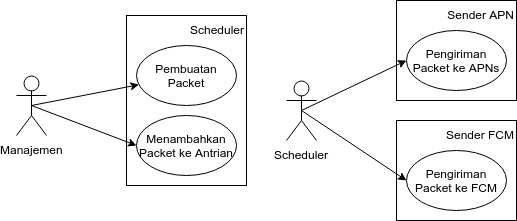
\includegraphics[width=1\textwidth]{bab3/figures/diagram_kasus_penggunaan.jpg}
    \caption{Diagram Kasus Penggunaan}
    \label{diagram_kasus_penggunaan}
\end{figure}
Penjelasan lebih lengkap dapat dilihat pada tabel~\ref{tabel_deskripsi_kasus_penggunaan_sistem}.
\begin{longtable}{|p{1cm}|p{5.5cm}|p{2cm}|}
    \hline
    \textbf{Kode} & \textbf{Nama Kasus Penggunaan} & \textbf{Aktor} & \hline
    UC01 & Pembuatan Packet & Scheduler & \hline
    UC02 & Menambahkan Packet ke Antrian & Scheduler & \hline
    UC03 & Pengiriman Packet ke APNs & Sender APN & \hline
    UC04 & Pengiriman Packet ke FCM & Sender FCM & \hline
    \caption{Deskripsi Kasus Penggunaan Sistem}
    \label{tabel_deskripsi_kasus_penggunaan_sistem}
\end{longtable}

% template tabel deskripsi kasus penggunaan
\newcommand\tableUcDesc[7] {
\begin{longtable}{|p{2.5cm}|p{6.5cm}|}
    \hline
    \textbf{Komponen} & \textbf{Deskripsi} & \hline
    Kode & #1 & \hline
    Nama & #2 & \hline
    Deskripsi & #3 & \hline
    Aktor & #4 & \hline
    Kondisi Awal & #5 & \hline
    Kondisi Akhir & #6 & \hline
    Alur Normal & #7 & \hline
    \caption{Kasus Penggunaan #2}
\end{longtable}
}

\paragraph{Pembuatan Packet}
\par Pada kasus ini, \textit{Scheduler} akan memeriksa secara berkala apakah terdapat batch yang belum di proses.
Jika ada, \textit{Scheduler} akan membuatkan \textit{packet} untuk \textit{batch} tersebut.
\tableUcDesc
{UC01}
{Pembuatan Packet}
{Packet akan dibuat setiap ada batch baru di database}
{Scheduler}
{Batch ditambahkan ke database}
{Packet ditambahkan ke database}
{
\begin{enumerate}
    \item Aktor memeriksa apakah terdapat batch yang belum di proses di database.
    \item Aktor membuat data packet dari data batch tersebut.
    \item Aktor menyimpan data packet dan memperbarui data batch di database.
\end{enumerate}
}

\paragraph{Menambahkan Packet ke Antrian}
\par Pada kasus ini, Scheduler akan memeriksa pada interval waktu tertentu apakah ada packet yang sudah waktunya untuk
dikirim.
Jika ada, scheduler akan menambahkan packet tersebut ke antrian kafka dengan topik yang sesuai.
\tableUcDesc
{UC02}
{Menambahkan Packet ke Antrian}
{Packet akan diantrikan ke kafka sesuai dengan jadwal pengiriman dan topik (Android, Web, atau iOS)}
{Scheduler}
{1 menit setelah pengecekan terakhir}
{Packet diantrikan ke kafka}
{
\begin{enumerate}
    \item Aktor memeriksa apakah terdapat packet yang sudah waktunya dikirim di database.
    \item Aktor menambahkan packet ke dalam antrian kafka dengan spesifikasi topik sebagai berikut:
    \begin{enumerate}
        \item Topik "android" untuk packet dengan target perangkat Android.
        \item Topik "web" untuk packet dengan target perangkat Web.
        \item Topik "ios" untuk packet dengan target perangkat iOS.
    \end{enumerate}
    \item Aktor memperbarui data packet di database.
\end{enumerate}
}

\paragraph{Pengiriman Packet ke APNs}
\par Pada kasus ini, Sender APN akan menunggu Kafka untuk mengirimkan packet yang berada dalam antrian topik "ios".
Setelah packet diterima, packet akan dikirim ke layanan APNs, dan kemudian akan diterima oleh perangkat pengguna.
\tableUcDesc
{UC03}
{Pengiriman Packet ke APNs}
{Packet yang ada didalam antrian topik "ios" akan dikirimkan ke layanan APNs}
{Sender APN}
{Packet diterima dari antrian topik "ios" di Kafka}
{Packet diterima oleh APNs}
{
\begin{enumerate}
    \item Aktor menunggu packet dari antrian topik "ios" di kafka.
    \item Aktor mengirimkan request notifikasi ke layanan APNs berdasarkan data packet.
    \item Aktor memperbarui data packet di database berdasarkan response dari APNs.
\end{enumerate}
}

\paragraph{Pengiriman Packet ke FCM}
\par Pada kasus ini, Sender FCM akan menunggu Kafka untuk mengirimkan packet yang berada dalam antrian topik "android" dan "web".
Setelah packet diterima, packet akan dikirim ke layanan FCM, dan kemudian akan diterima oleh perangkat pengguna.
\tableUcDesc
{UC04}
{Pengiriman Packet ke FCM}
{Packet yang ada didalam antrian topik "android" akan dikirimkan ke layanan FCM}
{Sender FCM}
{Packet diterima dari antrian topik "android" atau "web" di kafka}
{Packet diterima oleh FCM}
{
\begin{enumerate}
    \item Aktor menunggu packet dari antrian topik "android" atau "web" di kafka.
    \item Aktor mengirimkan request notifikasi ke layanan FCM berdasarkan data packet.
    \item Aktor memperbarui data packet di database berdasarkan response dari FCM.
\end{enumerate}
}

\section{Perancangan Sistem}
\par Subbab ini akan membahas tahapan perancangan sistem yang dibagi menjadi beberapa bagian, yaitu perancangan
arsitektur, data, dan proses.

\subsection{Perancangan Arsitektur}
\par Aplikasi \textit{push notification} terpusat akan dibagi menjadi 3 modul, yaitu \textit{Scheduler},
\textit{Sender APN}, dan \textit{Sender FCM}.
Aplikasi dibangun dengan bahasa pemrograman Java, dengan kerangka kerja
Spring.
Aplikasi saling terhubung lewat Kafka dan SQL Server.
Secara garis besar, aplikasi ini memiliki rancangan
arsitektur pengiriman notifikasi yang dapat dilihat pada gambar~\ref{arsitektur_pengiriman_notifikasi}.
\begin{figure}[H]
    \centering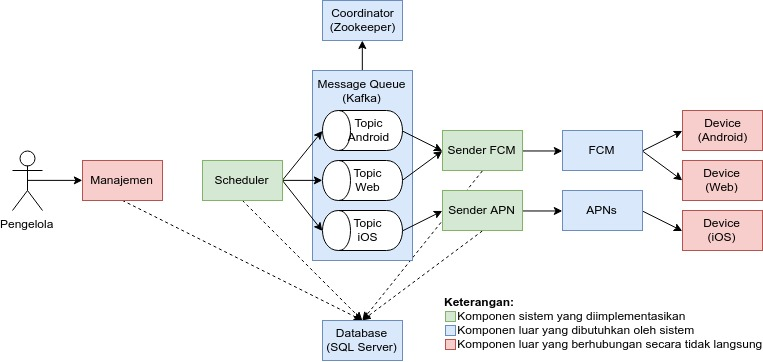
\includegraphics[width=1\textwidth]{bab3/figures/arsitektur_pengiriman_notifikasi.jpg}
    \caption{Arsitektur Pengiriman Notifikasi}
    \label{arsitektur_pengiriman_notifikasi}
\end{figure}

\subsection{Perancangan Basis Data}
\par Subbab ini membahas bagaimana rancangan basis data yang digunakan pada aplikasi \textit{push notification}
terpusat.
Basis data yang digunakan adalah SQL Server 2012.

\subsubsection{Tabel User (user\_account)}
\par Tabel ini digunakan untuk menyimpan data pengguna aplikasi yang ada di Institut Teknologi Sepuluh Nopember. Detail atribut dapat dilihat pada tabel berikut.
\begin{longtable}{|p{2.5cm}|p{2cm}|p{4.5cm}|}
    \hline
    \textbf{Nama Atribut} & \textbf{Tipe Data} & \textbf{Deskripsi} & \hline
    User ID & uuid & Primary key tabel & \hline
    Created At & datetime & Tanggal dan waktu dibuat & \hline
    Update At & datetime & Tanggal dan waktu diperbarui & \hline
    \caption{Tabel User (user\_account)}
\end{longtable}

\subsubsection{Tabel Group (pn\_group)}
\par Tabel ini digunakan untuk mengelompokan pengguna. Detail atribut dapat dilihat pada tabel berikut.
\begin{longtable}{|p{2.5cm}|p{2cm}|p{4.5cm}|}
    \hline
    \textbf{Nama Atribut} & \textbf{Tipe Data} & \textbf{Deskripsi} & \hline
    Group ID & uuid & Primary key tabel & \hline
    Created At & datetime & Tanggal dan waktu dibuat & \hline
    Update At & datetime & Tanggal dan waktu diperbarui & \hline
    \caption{Tabel Group (pn\_group)}
\end{longtable}

\subsubsection{Tabel Group Member (pn\_group\_member)}
\par Tabel ini digunakan untuk menambahkan pengguna kedalam suatu kelompok. Detail atribut dapat dilihat pada tabel berikut.
\begin{longtable}{|p{2.5cm}|p{2cm}|p{4.5cm}|}
    \hline
    \textbf{Nama Atribut} & \textbf{Tipe Data} & \textbf{Deskripsi} & \hline
    Group ID & uuid & Grup tempat pengguna terdaftar & \hline
    User ID & uuid & Pengguna yang terdaftar di grup & \hline
    Created At & datetime & Tanggal dan waktu dibuat & \hline
    Update At & datetime & Tanggal dan waktu diperbarui & \hline
    \caption{Tabel Group Member (pn\_group\_member)}
\end{longtable}

\subsubsection{Tabel Client (oauth\_client)}
\par Tabel ini digunakan untuk menyimpan data \textit{client} (aplikasi) yang ada di Institut Teknologi Sepuluh Nopember. Detail atribut dapat dilihat pada tabel berikut.
\begin{longtable}{|p{2.5cm}|p{2cm}|p{4.5cm}|}
    \hline
    \textbf{Nama Atribut} & \textbf{Tipe Data} & \textbf{Deskripsi} & \hline
    Client ID & uuid & Primary key tabel & \hline
    Created At & datetime & Tanggal dan waktu dibuat & \hline
    Update At & datetime & Tanggal dan waktu diperbarui & \hline
    \caption{Tabel Client (oauth\_client)}
\end{longtable}

\subsubsection{Tabel Certificate (pn\_certificate)}
\par Tabel ini digunakan untuk menyimpan data sertifikat yang digunakan untuk autentikasi ke layanan APNs dan FCM. Detail atribut dapat dilihat pada tabel berikut.
\begin{longtable}{|p{2.5cm}|p{2cm}|p{4.5cm}|}
    \hline
    \textbf{Nama Atribut} & \textbf{Tipe Data} & \textbf{Deskripsi} & \hline
    Certificate ID & uuid & Primary key tabel & \hline
    Client ID & uuid & Foreign key tabel client & \hline
    Bundle ID & varchar(255) & Bundle ID untuk aplikasi iOS & \hline
    Certificate Key & text & File sertifikat yang sudah diencode dengan base64 & \hline
    Type & char(1) & Tipe sertifikat (FCM atau APNs) & \hline
    Password & varchar(255) & Kata sandi untuk sertifikat iOS & \hline
    Created At & datetime & Tanggal dan waktu dibuat & \hline
    Update At & datetime & Tanggal dan waktu diperbarui & \hline
    \caption{Tabel Certificate (pn\_certificate)}
\end{longtable}

\subsubsection{Tabel Device (device\_token)}
\par Tabel ini digunakan untuk menyimpan data perangkat pengguna yang terdaftar di layanan APNs dan FCM. Detail atribut dapat dilihat pada tabel berikut.
\begin{longtable}{|p{2.5cm}|p{2cm}|p{4.5cm}|}
    \hline
    \textbf{Nama Atribut} & \textbf{Tipe Data} & \textbf{Deskripsi} & \hline
    Device ID & uuid & Primary key tabel & \hline
    Client ID & uuid & Client tempat perangkat terdaftar & \hline
    User ID & uuid & User pemilik perangkat & \hline
    Device Token & varchar(255) & Token yang terdaftar di layanan APNs dan FCM & \hline
    Device Type & char(1) & Jenis perangkat (Android, Web, atau iOS) & \hline
    Active & numeric(1) & Perangkat aktif atau tidak & \hline
    Created At & datetime & Tanggal dan waktu dibuat & \hline
    Update At & datetime & Tanggal dan waktu diperbarui & \hline
    \caption{Tabel Device (device\_token)}
\end{longtable}

\subsubsection{Tabel Batch (pn\_batch)}
\par Tabel ini digunakan untuk menyimpan data notifikasi yang akan dikirim ke beberapa perangkat. Detail atribut dapat dilihat pada tabel berikut.
\begin{longtable}{|p{2.5cm}|p{2cm}|p{4.5cm}|}
    \hline
    \textbf{Nama Atribut} & \textbf{Tipe Data} & \textbf{Deskripsi} & \hline
    Batch ID & uuid & Primary key tabel & \hline
    Title & varchar(255) & Judul notifikasi & \hline
    Body & varchar(255) & Isi pesan notifikasi & \hline
    Image & varchar(255) & Nama atau URL Gambar & \hline
    Sound & varchar(255) & Nama atau URL Suara & \hline
    Action & varchar(255) & Nama aksi yang dijalankan jika notifikasi dibuka & \hline
    Additional Data & varchar(255) & Data tambahan dengan format JSON & \hline
    Delivery Date & datetime & Waktu notifikasi dikirim & \hline
    Started Date & datetime & Waktu batch mulai diproses & \hline
    Finished Date & datetime & Waktu batch selesai diproses & \hline
    Is Allowed & numeric(1) & Batch boleh diproses atau tidak & \hline
    User Sender ID & uuid & User pembuat batch & \hline
    Client Sender ID & uuid & Client pembuat batch & \hline
    Client Destination ID & uuid & Client tujuan penerima notifikasi & \hline
    Created At & datetime & Tanggal dan waktu dibuat & \hline
    Update At & datetime & Tanggal dan waktu diperbarui & \hline
    \caption{Tabel Batch (pn\_batch)}
\end{longtable}

\subsubsection{Tabel Packet (pn\_packet)}
\par Tabel ini digunakan untuk menyimpan data notifikasi yang dikirim ke satu perangkat. Detail atribut dapat dilihat pada tabel berikut.
\begin{longtable}{|p{2.5cm}|p{2cm}|p{4.5cm}|}
    \hline
    \textbf{Nama Atribut} & \textbf{Tipe Data} & \textbf{Deskripsi} & \hline
    Packet ID & uuid & Primary key tabel & \hline
    Batch ID & uuid & Batch notifikasi & \hline
    Device Token ID & uuid & Perangkat penerima notifikasi & \hline
    Sent At & datetime & Waktu notifikasi diterima oleh APNs atau FCM & \hline
    Reason & varchar(255) & Penyebab jika terjadi kegagalan & \hline
    Packet Status & numeric(1) & Status pengiriman packet (dibuat, menunggu, berhasil, atau gagal) & \hline
    Created At & datetime & Tanggal dan waktu dibuat & \hline
    Update At & datetime & Tanggal dan waktu diperbarui & \hline
    \caption{Tabel Packet (pn\_packet)}
\end{longtable}

\subsubsection{Tabel User Destination (pn\_user\_destination)}
\par Tabel ini digunakan untuk menyimpan data pengguna yang menjadi target penerima notifikasi dalam satu \textit{batch}. Detail atribut dapat dilihat pada tabel berikut.
\begin{longtable}{|p{2.5cm}|p{2cm}|p{4.5cm}|}
    \hline
    \textbf{Nama Atribut} & \textbf{Tipe Data} & \textbf{Deskripsi} & \hline
    Batch ID & uuid & Batch notifikasi & \hline
    User ID & uuid & Pengguna penerima notifikasi & \hline
    Created At & datetime & Tanggal dan waktu dibuat & \hline
    Update At & datetime & Tanggal dan waktu diperbarui & \hline
    \caption{Tabel User Destination (pn\_user\_destination)}
\end{longtable}

\subsubsection{Tabel Group Destination (pn\_group\_destination)}
\par Tabel ini digunakan untuk menyimpan data kelompok yang menjadi target penerima notifikasi dalam satu \textit{batch}. Detail atribut dapat dilihat pada tabel berikut.
\begin{longtable}{|p{2.5cm}|p{2cm}|p{4.5cm}|}
    \hline
    \textbf{Nama Atribut} & \textbf{Tipe Data} & \textbf{Deskripsi} & \hline
    Batch ID & uuid & Batch notifikasi & \hline
    Group ID & uuid & Grup penerima notifikasi & \hline
    Created At & datetime & Tanggal dan waktu dibuat & \hline
    Update At & datetime & Tanggal dan waktu diperbarui & \hline
    \caption{Tabel Group Destination (pn\_group\_destination)}
\end{longtable}

\subsection{Perancangan Proses}
\par Subbab ini menjelaskan tentang rancangan, tujuan, dan diagram alir proses-proses yang ada pada aplikasi
\textit{push notification} terpusat.

\subsubsection{Proses Pembuatan Packet}
\par Proses ini bertujuan untuk membuat \textit{packet} dari \textit{batch} yang baru dibuat.
Proses pembuatan dapat
dilihat di diagram alir pada gambar~\ref{flowchart_pembuatan_packet}.
\begin{figure}[H]
    \centering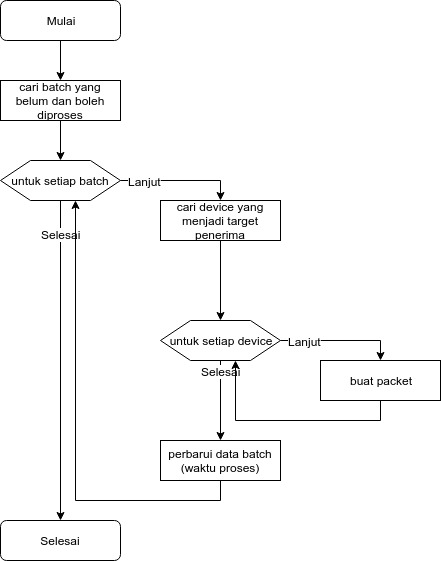
\includegraphics[width=0.8\textwidth]{bab3/figures/flowchart_pembuatan_packet.jpg}
    \caption{Diagram Alir Proses Pembuatan \textit{Packet}}
    \label{flowchart_pembuatan_packet}
\end{figure}

\subsubsection{Proses Menambahkan Packet ke Antrian}
\par Proses ini bertujuan untuk mengantrikan \textit{packet} yang sudah waktunya untuk dikirim.
Antrian
\textit{packet} dibagi berdasarkan jenis perangkat penerima notifikasi (Android, Web, atau iOS).
Proses pengantrian
dapat dilihat di diagram alir pada gambar~\ref{flowchart_menambahkan_packet_ke_antrian}.
\begin{figure}[H]
    \centering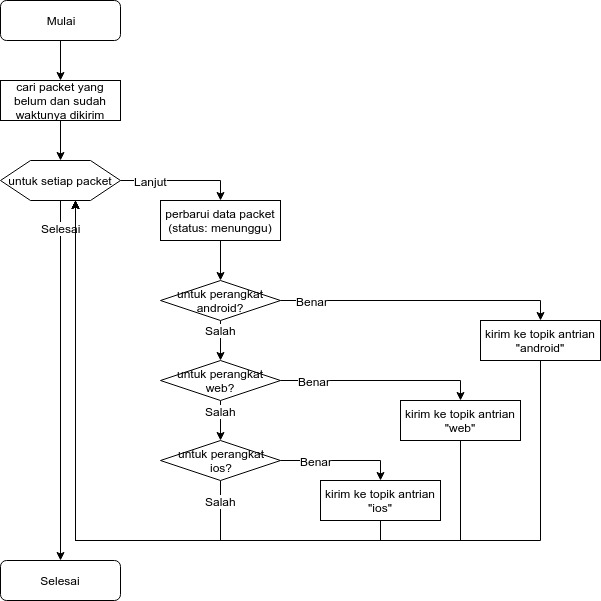
\includegraphics[width=0.7\textwidth]{bab3/figures/flowchart_menambahkan_packet_ke_antrian.jpg}
    \caption{Diagram Alir Proses Menambahkan \textit{Packet} ke Antrian}
    \label{flowchart_menambahkan_packet_ke_antrian}
\end{figure}

\subsubsection{Proses Pengiriman Packet ke APNs}
\par Proses ini bertujuan untuk mengirimkan \textit{packet} yang ada di antrian topik "ios" ke perangkat pengguna
yang berbasis iOS lewat layanan APNs. Proses pengiriman \textit{packet} dapat dilihat di diagram alir pada
gambar~\ref{flowchart_pengiriman_packet_ke_apns}.
\begin{figure}[H]
    \centering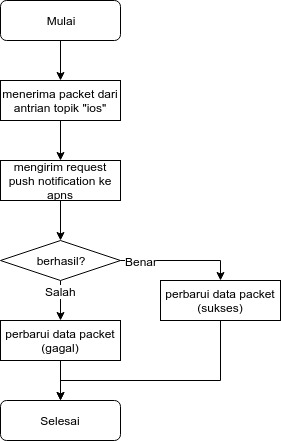
\includegraphics[width=0.7\textwidth]{bab3/figures/flowchart_pengiriman_packet_ke_apns.jpg}
    \caption{Diagram Alir Proses Pengiriman \textit{Packet} ke APNs}
    \label{flowchart_pengiriman_packet_ke_apns}
\end{figure}
\linebreak

\subsubsection{Proses Pengiriman Packet ke FCM}
\par Proses ini bertujuan untuk mengirimkan \textit{packet} yang ada di antrian topik "android" dan "web" ke
perangkat pengguna yang berbasis Android atau Web lewat layanan FCM. Proses pengiriman \textit{packet} dapat dilihat di
diagram alir pada gambar~\ref{flowchart_pengiriman_packet_ke_fcm}.
\begin{figure}[H]
    \centering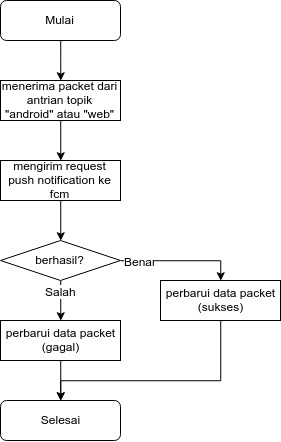
\includegraphics[width=0.7\textwidth]{bab3/figures/flowchart_pengiriman_packet_ke_fcm.jpg}
    \caption{Diagram Alir Proses Pengiriman \textit{Packet} ke FCM}
    \label{flowchart_pengiriman_packet_ke_fcm}
\end{figure}
\linebreak
 \cleardoublepage
    \chapter {IMPLEMENTASI}
\par Bab ini membahas implementasi dari rancangan sistem yang ada pada bab 3. Bahasa pemrograman yang digunakan untuk implementasi aplikasi \textit{push notification}.

\section{Lingkungan Implementasi}
\par Lingkungan implementasi yang digunakan untuk mengembangkan tugas akhir ini memiliki spesifikasi perangkat keras dan lunak seperti ditampilkan pada Tabel \ref{tabel_spesifikasi_server}, Tabel \ref{tabel_spesifikasi_perangkat_android}, dan Tabel \ref{tabel_spesifikasi_perangkat_ios}.
\begin{table}[H]
	\centering
	\begin{tabularx}{0.75\textwidth}{|l|X|}
		\hline
		\textbf{Jenis} & \textbf{Spesifikasi} \\ \hline
		CPU & AMD Ryzen 5 2500U \\ \hline
		CPU Core & 4 \\ \hline
		Memory & 12 GB \\ \hline
		Sistem Operasi & Ubuntu 19.04 \\ \hline
		IDE & Intellij IDEA \\ \hline
	\end{tabularx}
	\caption{Spesifikasi Server}
	\label{tabel_spesifikasi_server}
\end{table}
\begin{table}[H]
	\centering
	\begin{tabularx}{0.75\textwidth}{|l|X|}
		\hline
		\textbf{Jenis} & \textbf{Spesifikasi} \\ \hline
		CPU & Snapdragon 636 \\ \hline
		Memory & 3 GB \\ \hline
		Sistem Operasi & Android 9 (Pie) \\ \hline
	\end{tabularx}
	\caption{Spesifikasi Perangkat Android}
	\label{tabel_spesifikasi_perangkat_android}
\end{table}
\begin{table}[H]
	\centering
	\begin{tabularx}{0.75\textwidth}{|l|X|}
		\hline
		\textbf{Jenis} & \textbf{Spesifikasi} \\ \hline
		CPU & Apple A10 Fusion \\ \hline
		Memory & 3 GB \\ \hline
		Sistem Operasi & iOS 12 \\ \hline
	\end{tabularx}
	\caption{Spesifikasi Perangkat iOS}
	\label{tabel_spesifikasi_perangkat_ios}
\end{table}

\section{Implementasi Basis Data}
\par Subbab ini membahas struktur tabel yang digunakan, meliputi tujuan pembuatan tabel, Kode yang digunakan untuk membuat tabel, dan gambar tabel yang telah dibuat.

\subsection{Implementasi Tabel User}
\par Tabel user digunakan untuk menyimpan data pengguna. Kode yang digunakan untuk membuat tabel dapat dilihat pada Kode Sumber \ref{code:user_account} dan hasil tabel dapat dilihat pada Gambar \ref{tabel_user_account}.
\lstinputlisting[label=code:user_account, caption=Implementasi Tabel User, language=SQL]{bab4/codes/user_account.sql}
\begin{figure}[H]
    \centering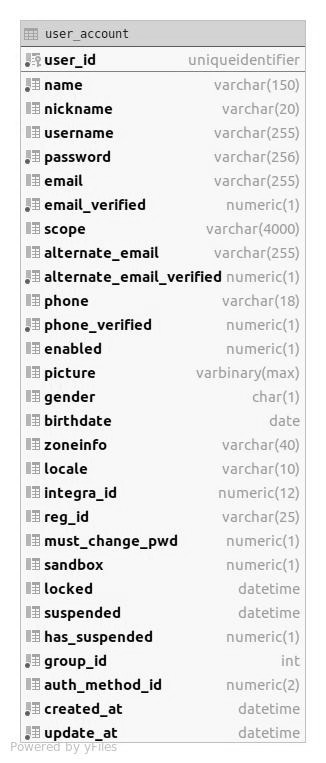
\includegraphics[width=0.5\textwidth]{bab4/figures/tabel_user_account.jpg}
    \caption{Tabel User (user\_account)}
    \label{tabel_user_account}
\end{figure}

\subsection{Implementasi Tabel Group}
\par Tabel group digunakan untuk menyimpan data kelompok pengguna. Kode yang digunakan untuk membuat tabel dapat dilihat pada Kode Sumber \ref{code:pn_group} dan hasil tabel dapat dilihat pada Gambar \ref{tabel_pn_group}.
\lstinputlisting[label=code:pn_group, caption=Implementasi Tabel Group, language=SQL]{bab4/codes/pn_group.sql}
\begin{figure}[H]
    \centering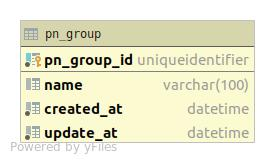
\includegraphics[width=0.5\textwidth]{bab4/figures/tabel_pn_group.jpg}
    \caption{Tabel Group (pn\_group)}
    \label{tabel_pn_group}
\end{figure}

\subsection{Implementasi Tabel Group Member}
\par Tabel group member digunakan untuk menyimpan data anggota kelompok pengguna. Kode yang digunakan untuk membuat tabel dapat dilihat pada Kode Sumber \ref{code:pn_group_member} dan hasil tabel dapat dilihat pada Gambar \ref{tabel_pn_group_member}.
\lstinputlisting[label=code:pn_group_member, caption=Implementasi Tabel Group Member, language=SQL]{bab4/codes/pn_group_member.sql}
\begin{figure}[H]
    \centering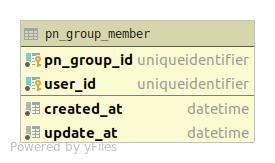
\includegraphics[width=0.5\textwidth]{bab4/figures/tabel_pn_group_member.jpg}
    \caption{Tabel Group Member (pn\_group\_member)}
    \label{tabel_pn_group_member}
\end{figure}

\subsection{Implementasi Tabel Client}
\par Tabel client digunakan untuk menyimpan data aplikasi. Kode yang digunakan untuk membuat tabel dapat dilihat pada Kode Sumber \ref{code:oauth_client} dan hasil tabel dapat dilihat pada Gambar \ref{tabel_oauth_client}.
\lstinputlisting[label=code:oauth_client, caption=Implementasi Tabel Client, language=SQL]{bab4/codes/oauth_client.sql}
\begin{figure}[H]
    \centering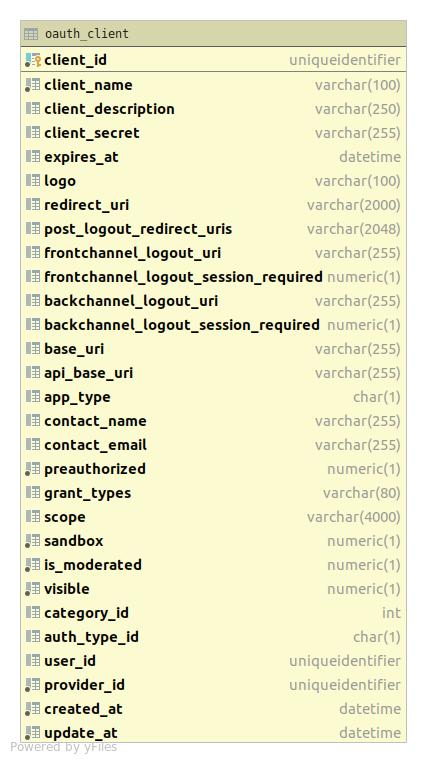
\includegraphics[width=0.5\textwidth]{bab4/figures/tabel_oauth_client.jpg}
    \caption{Tabel Client (oauth\_client)}
    \label{tabel_oauth_client}
\end{figure}

\subsection{Implementasi Tabel Certificate}
\par Tabel certificate digunakan untuk menyimpan data sertifikat client untuk autentikasi ke layanan APNs dan FCM. Kode yang digunakan untuk membuat tabel dapat dilihat pada Kode Sumber \ref{code:pn_certificate} dan hasil tabel dapat dilihat pada Gambar \ref{tabel_pn_certificate}.
\lstinputlisting[label=code:pn_certificate, caption=Implementasi Tabel Certificate, language=SQL]{bab4/codes/pn_certificate.sql}
\begin{figure}[H]
    \centering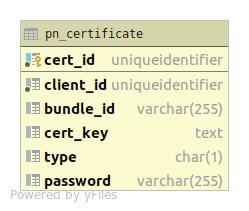
\includegraphics[width=0.5\textwidth]{bab4/figures/tabel_pn_certificate.jpg}
    \caption{Tabel Certificate (pn\_certificate)}
    \label{tabel_pn_certificate}
\end{figure}

\subsection{Implementasi Tabel Device}
\par Tabel device digunakan untuk menyimpan data perangkat pengguna yang terdaftar di layanan APNs dan FCM. Kode yang digunakan untuk membuat tabel dapat dilihat pada Kode Sumber \ref{code:device_token} dan hasil tabel dapat dilihat pada Gambar \ref{tabel_device_token}.
\lstinputlisting[label=code:device_token, caption=Implementasi Tabel Device, language=SQL]{bab4/codes/device_token.sql}
\begin{figure}[H]
    \centering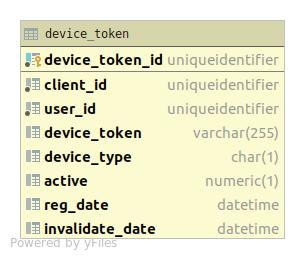
\includegraphics[width=0.5\textwidth]{bab4/figures/tabel_device_token.jpg}
    \caption{Tabel Device (device\_token)}
    \label{tabel_device_token}
\end{figure}

\subsection{Implementasi Tabel Batch}
\par Tabel batch digunakan untuk menyimpan data notifikasi yang akan dikirim ke beberapa pengguna atau kelompok. Kode yang digunakan untuk membuat tabel dapat dilihat pada Kode Sumber \ref{code:pn_batch} dan hasil tabel dapat dilihat pada Gambar \ref{tabel_pn_batch}.
\lstinputlisting[label=code:pn_batch, caption=Implementasi Tabel Batch, language=SQL]{bab4/codes/pn_batch.sql}
\begin{figure}[H]
    \centering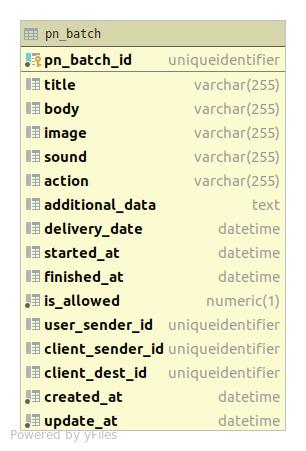
\includegraphics[width=0.5\textwidth]{bab4/figures/tabel_pn_batch.jpg}
    \caption{Tabel Batch (pn\_batch)}
    \label{tabel_pn_batch}
\end{figure}

\subsection{Implementasi Tabel Packet}
\par Tabel packet digunakan untuk menyimpan data notifikasi yang akan dikirim ke satu perangkat. Kode yang digunakan untuk membuat tabel dapat dilihat pada Kode Sumber \ref{code:pn_packet} dan hasil tabel dapat dilihat pada Gambar \ref{tabel_pn_packet}.
\lstinputlisting[label=code:pn_packet, caption=Implementasi Tabel Packet, language=SQL]{bab4/codes/pn_packet.sql}
\begin{figure}[H]
    \centering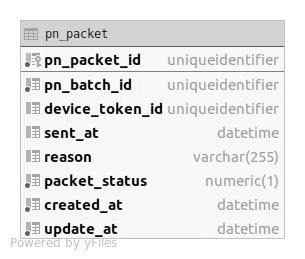
\includegraphics[width=0.5\textwidth]{bab4/figures/tabel_pn_packet.jpg}
    \caption{Tabel Packet (pn\_packet)}
    \label{tabel_pn_packet}
\end{figure}

\subsection{Implementasi Tabel User Destination}
\par Tabel user destination digunakan untuk menyimpan data pengguna yang akan menerima notifikasi dari suatu batch. Kode yang digunakan untuk membuat tabel dapat dilihat pada Kode Sumber \ref{code:pn_user_destination} dan hasil tabel dapat dilihat pada Gambar \ref{tabel_pn_user_destination}.
\lstinputlisting[label=code:pn_user_destination, caption=Implementasi Tabel User Destination, language=SQL]{bab4/codes/pn_user_destination.sql}
\begin{figure}[H]
    \centering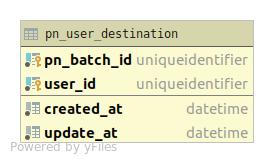
\includegraphics[width=0.5\textwidth]{bab4/figures/tabel_pn_user_destination.jpg}
    \caption{Tabel User Destination (pn\_user\_destination)}
    \label{tabel_pn_user_destination}
\end{figure}

\subsection{Implementasi Tabel Group Destination}
\par Tabel group destination digunakan untuk menyimpan data kelompok yang akan menerima notifikasi dari suatu batch. Kode yang digunakan untuk membuat tabel dapat dilihat pada Kode Sumber \ref{code:pn_group_destination} dan hasil tabel dapat dilihat pada Gambar \ref{tabel_pn_group_destination}.
\lstinputlisting[label=code:pn_group_destination, caption=Implementasi Tabel Group Destination, language=SQL]{bab4/codes/pn_group_destination.sql}
\begin{figure}[H]
    \centering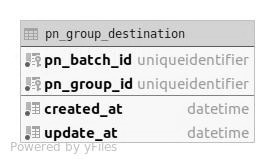
\includegraphics[width=0.5\textwidth]{bab4/figures/tabel_pn_group_destination.jpg}
    \caption{Tabel Group Destination (pn\_group\_destination)}
    \label{tabel_pn_group_destination}
\end{figure}

\section{Implementasi Message Queue}
%TODO

\subsection{Implementasi Kafka}
%TODO

\subsection{Implementasi Zookeeper}
%TODO

%TODO kopas kodingan
\section{Implementasi Proses dan Kasus Penggunaan}
\par Subbab ini membahas implementasi proses yang dibuat berdasarkan hasil analisa dan rancangan yang telah dilakukan.

\subsection{Implementasi Pembuatan Packet}
\par Proses pembuatan \textit{packet} dilakukan secara berkala oleh modul Scheduler setiap 30 detik. \textit{Packet} yang telah dibuat akan disimpan ke SQL Server. Hasil implementasi dapat dilihat pada Kode Sumber \ref{code:pembuatan_packet}.
\lstinputlisting[label=code:pembuatan_packet, caption=Implementasi Pembuatan Packet, language=Java] {bab4/codes/pembuatan_packet.java}

\subsubsection{Implementasi Menambahkan Packet ke Antrian}
\par Proses menambahkan \textit{packet} ke antrian dilakukan secara berkala oleh modul Scheduler setiap 30 detik dengan jeda awal 15 detik. Tujuan penambahan jeda awal adalah untuk mengoptimalkan penggunaan sumber daya \textit{server} dengan mencegah proses pembuatan dan mengantrikan packet berjalan bersamaan. \textit{Packet} yang siap dikirim akan diantrikan ke Kafka. Hasil implementasi dapat dilihat pada Kode Sumber \ref{code:menambahkan_packet_ke_antrian}.
\lstinputlisting[label=code:menambahkan_packet_ke_antrian, caption=Implementasi Menambahkan Packet ke Antrian, language=Java] {bab4/codes/menambahkan_packet_ke_antrian.java}

\subsection{Implementasi Pengiriman Packet ke APNs}
\par Proses pengiriman \textit{packet} ke APNs dilakukan secara berkala oleh Sender APN dengan cara menunggu Kafka untuk memberikan \textit{packet} yang berada diantrian topik "ios". Hasil implementasi dapat dilihat pada Kode Sumber \ref{code:pengiriman_packet_ke_apns}.
\lstinputlisting[label=code:pengiriman_packet_ke_apns, caption=Implementasi Pengiriman Packet ke APNs, language=Java] {bab4/codes/pengiriman_packet_ke_apns.java}

\subsection{Implementasi Pengiriman Packet ke FCM}
\par Proses pengiriman packet dilakukan secara berkala oleh Sender FCM dengan cara menunggu Kafka untuk mengirimkan data packet yang berada diantrian topik "android" dan "web". Hasil implementasi dapat dilihat pada Kode Sumber \ref{code:pengiriman_packet_ke_fcm}.
\lstinputlisting[label=code:pengiriman_packet_ke_fcm, caption=Implementasi Pengiriman Packet ke FCM, language=Java] {bab4/codes/pengiriman_packet_ke_fcm.java}

\subsection{Implementasi Pemantauan Aplikasi}
\par Proses pemantauan aplikasi (menampilkan penggunaan sumber daya, menampilkan status kesehatan, menampilkan konfigurasi, menampilkan log) diimplementasikan dengan menggunakan library Spring Boot Actuator dan Spring Boot Admin. Spring Boot Actuator digunakan untuk menampilkan hasil pemantauan dalam bentuk REST API, sementara Spring Boot Admin digunakan untuk menampilkan hasil pemantauan yang dilakukan oleh Spring Boot Actuator dalam bentuk halaman web. Potongan kode yang digunakan untuk konfigurasi Spring Boot Actuator dan Spring Boot Admin dapat dilihat pada kode sumber~X.
 \cleardoublepage
    \chapter{PENGUJIAN DAN EVALUASI}
\par Bab ini membahas pengujian dan evaluasi terhadap perangkat lunak yang telah diimplementasikan dengan menggunakan metode \textit{blackbox}.

\section{Lingkungan Pengujian}
\par Lingkungan yang digunakan untuk menguji tugas akhir ini memiliki spesifikasi perangkat keras dan lunak yang ditunjukkan pada Tabel \ref{t:spec-server}, \ref{t:spec-android}, \ref{t:spec-android-2}, \ref{t:spec-android-3} dan \ref{t:spec-ios}. Implementasi aplikasi android yang digunakan untuk pengujian dapat dilihat pada \nameref{lampiran:implementasi-android}.
\begin{longtable}{|p{3cm}|p{6cm}|}
	\caption{Spesifikasi Server} \label{t:spec-server} \\ \hline
    \rowcolor{lightgray} Komponen & Spesifikasi \\ \hline
    CPU & Intel(R) Xeon(R) CPU E5-2690 v4 \\ \hline
    CPU Core & 4 \\ \hline
    Memory & 8 GB \\ \hline
    Sistem Operasi & Ubuntu 18.04 \\ \hline
\end{longtable}
\begin{longtable}{|p{3cm}|p{6cm}|}
	\caption{Spesifikasi Perangkat Android 1} \label{t:spec-android} \\ \hline
	\rowcolor{lightgray} Komponen & Spesifikasi \\ \hline
    CPU & Snapdragon 636 \\ \hline
    Memory & 3 GB \\ \hline
    Sistem Operasi & Android 9 (Pie) \\ \hline
    Aplikasi & Push Notification Dev versi 1.0 \\ \hline
\end{longtable}
\pagebreak
\begin{longtable}{|p{3cm}|p{6cm}|}
\caption{Spesifikasi Perangkat Android 2} \label{t:spec-android-2} \\ \hline
\rowcolor{lightgray} Komponen & Spesifikasi \\ \hline
CPU & Snapdragon 625 \\ \hline
Memory & 4 GB \\ \hline
Sistem Operasi & Android 7 (Nougat) \\ \hline
Aplikasi & Push Notification Dev versi 1.0 \\ \hline
\end{longtable}
\begin{longtable}{|p{3cm}|p{6cm}|}
\caption{Spesifikasi Perangkat Android 3} \label{t:spec-android-3} \\ \hline
\rowcolor{lightgray} Komponen & Spesifikasi \\ \hline
CPU & Snapdragon 616 \\ \hline
Memory & 3 GB \\ \hline
Sistem Operasi & - \\ \hline
Aplikasi & Push Notification Dev versi 1.0 \\ \hline
\end{longtable}
\begin{longtable}{|p{3cm}|p{6cm}|}
	\caption{Spesifikasi Perangkat iOS} \label{t:spec-ios} \\ \hline
	\rowcolor{lightgray} Komponen & Spesifikasi \\ \hline
    CPU & Apple A10 Fusion \\ \hline
    Memory & 3 GB \\ \hline
    Sistem Operasi & iOS 12 \\ \hline
    Aplikasi & MyITS Wali versi 1.0.2 \\ \hline
\end{longtable}

\section{Pengujian Fungsional}
\par Pengujian fungsional dilakukan untuk mengetahui apakah sistem yang dibangun sudah memiliki kebutuhan fungsional yang diperlukan.

\subsection{Pengujian Pembuatan Packet}
\par Pengujian pembuatan \textit{packet} dilakukan untuk mengetahui apakah Scheduler berhasil membuatkan data \textit{packet} dari \textit{batch} dengan tepat. Hasil uji dapat dilihat pada Tabel \ref{t:uji_pembuatan_packet}.
\begin{longtable}{|>{\columncolor{lightgray}}p{3cm}|p{6.5cm}|}
	\caption{Hasil Uji Pembuatan \textit{Packet}} \label{t:uji_pembuatan_packet} \\ \hline
	Kode & FT-01 \\ \hline
	Nama & Pengujian Pembuatan \textit{Packet} \\ \hline
	Tujuan & Menguji apakah sistem mampu membuatkan data \textit{packet} dari data \textit{batch} \\ \hline
	Kondisi Awal & Scheduler aktif \\ \hline
	Langkah Pengujian &  
	\begin{enumerate}
		\item Pengguna menambahkan data \textit{batch} baru lewat halaman kirim notifikasi di modul manajemen.
		\item Setelah 30 detik, data \textit{packet} akan disimpan di sistem basis data.
	\end{enumerate} \\ \hline
	Hasil yang diharapkan & Data \textit{packet} tersimpan di sistem basis data \\ \hline
	Hasil yang diperoleh & Data \textit{packet} tersimpan di sistem basis data \\ \hline
	Hasil pengujian & Berhasil \\ \hline
\end{longtable}

\subsection{Pengujian Menambahkan Packet ke Antrian}
\par Pengujian menambahkan \textit{packet} dilakukan untuk mengetahui apakah Scheduler berhasil menambahkan \textit{packet} ke antrian dengan tepat. Hasil uji dapat dilihat pada Tabel \ref{t:uji_pembuatan_antrian}.
\begin{longtable}{|>{\columncolor{lightgray}}p{3cm}|p{6.5cm}|}
	\caption{Hasil Uji Menambahkan \textit{Packet} ke Antrian} \label{t:uji_pembuatan_antrian} \\ \hline
	Kode & FT-02 \\ \hline
	Nama & Pengujian Pembuatan Antrian \\ \hline
	Tujuan & Menguji apakah sistem mampu membuatkan data antrian dari data \textit{packet} \\ \hline
	Kondisi Awal & Scheduler aktif \\ \hline
	Langkah Pengujian &  
	\begin{enumerate}
		\item Pengguna menambahkan data \textit{batch} baru lewat halaman kirim notifikasi di modul manajemen.
		\item 30 detik setelah waktu pengiriman \textit{batch}, data \textit{packet} untuk \textit{batch} akan tersimpan di sistem antrian pesan.
	\end{enumerate} \\ \hline
	Hasil yang diharapkan & Data \textit{packet} tersimpan di sistem antrian pesan. \\ \hline
	Hasil yang diperoleh & Data \textit{packet} tersimpan di sistem antrian pesan. \\ \hline
	Hasil pengujian & Berhasil \\ \hline
\end{longtable}

\subsection{Pengujian Pengiriman Packet ke APNs}
\par Pengujian pengiriman \textit{packet} ke APNs dilakukan untuk mengetahui apakah Sender APN berhasil mengirimkan \textit{packet} ke layanan APNs dengan tepat. Hasil uji dan notifikasi dapat dilihat pada Tabel \ref{t:uji_pengiriman_packet_apn} dan Gambar \ref{f:ss_ios}.
\begin{longtable}{|>{\columncolor{lightgray}}p{3cm}|p{6.5cm}|}
	\caption{Hasil Uji Pengiriman \textit{Packet} ke APNs} \label{t:uji_pengiriman_packet_apn} \\ \hline
	Kode & FT-03 \\ \hline
	Nama & Pengujian Pembuatan \textit{Packet} \\ \hline
	Tujuan & Menguji apakah sistem mampu mengirim \textit{packet} lewat layanan APNs \\ \hline
	Kondisi Awal & Scheduler dan Sender APN aktif \\ \hline
	Langkah Pengujian &  
	\begin{enumerate}
		\item Pengguna menambahkan data \textit{batch} baru untuk perangkat iOS lewat halaman kirim notifikasi di modul Manajemen.
		\item 1 menit setelah waktu pengiriman \textit{batch}, notifikasi akan diterima oleh perangkat iOS.
	\end{enumerate} \\ \hline
	Hasil yang diharapkan & Notifikasi diterima oleh perangkat iOS \\ \hline
	Hasil yang diperoleh & Notifikasi diterima oleh perangkat iOS \\ \hline
	Hasil pengujian & Berhasil \\ \hline
\end{longtable}
\begin{figure}[H]
	\centering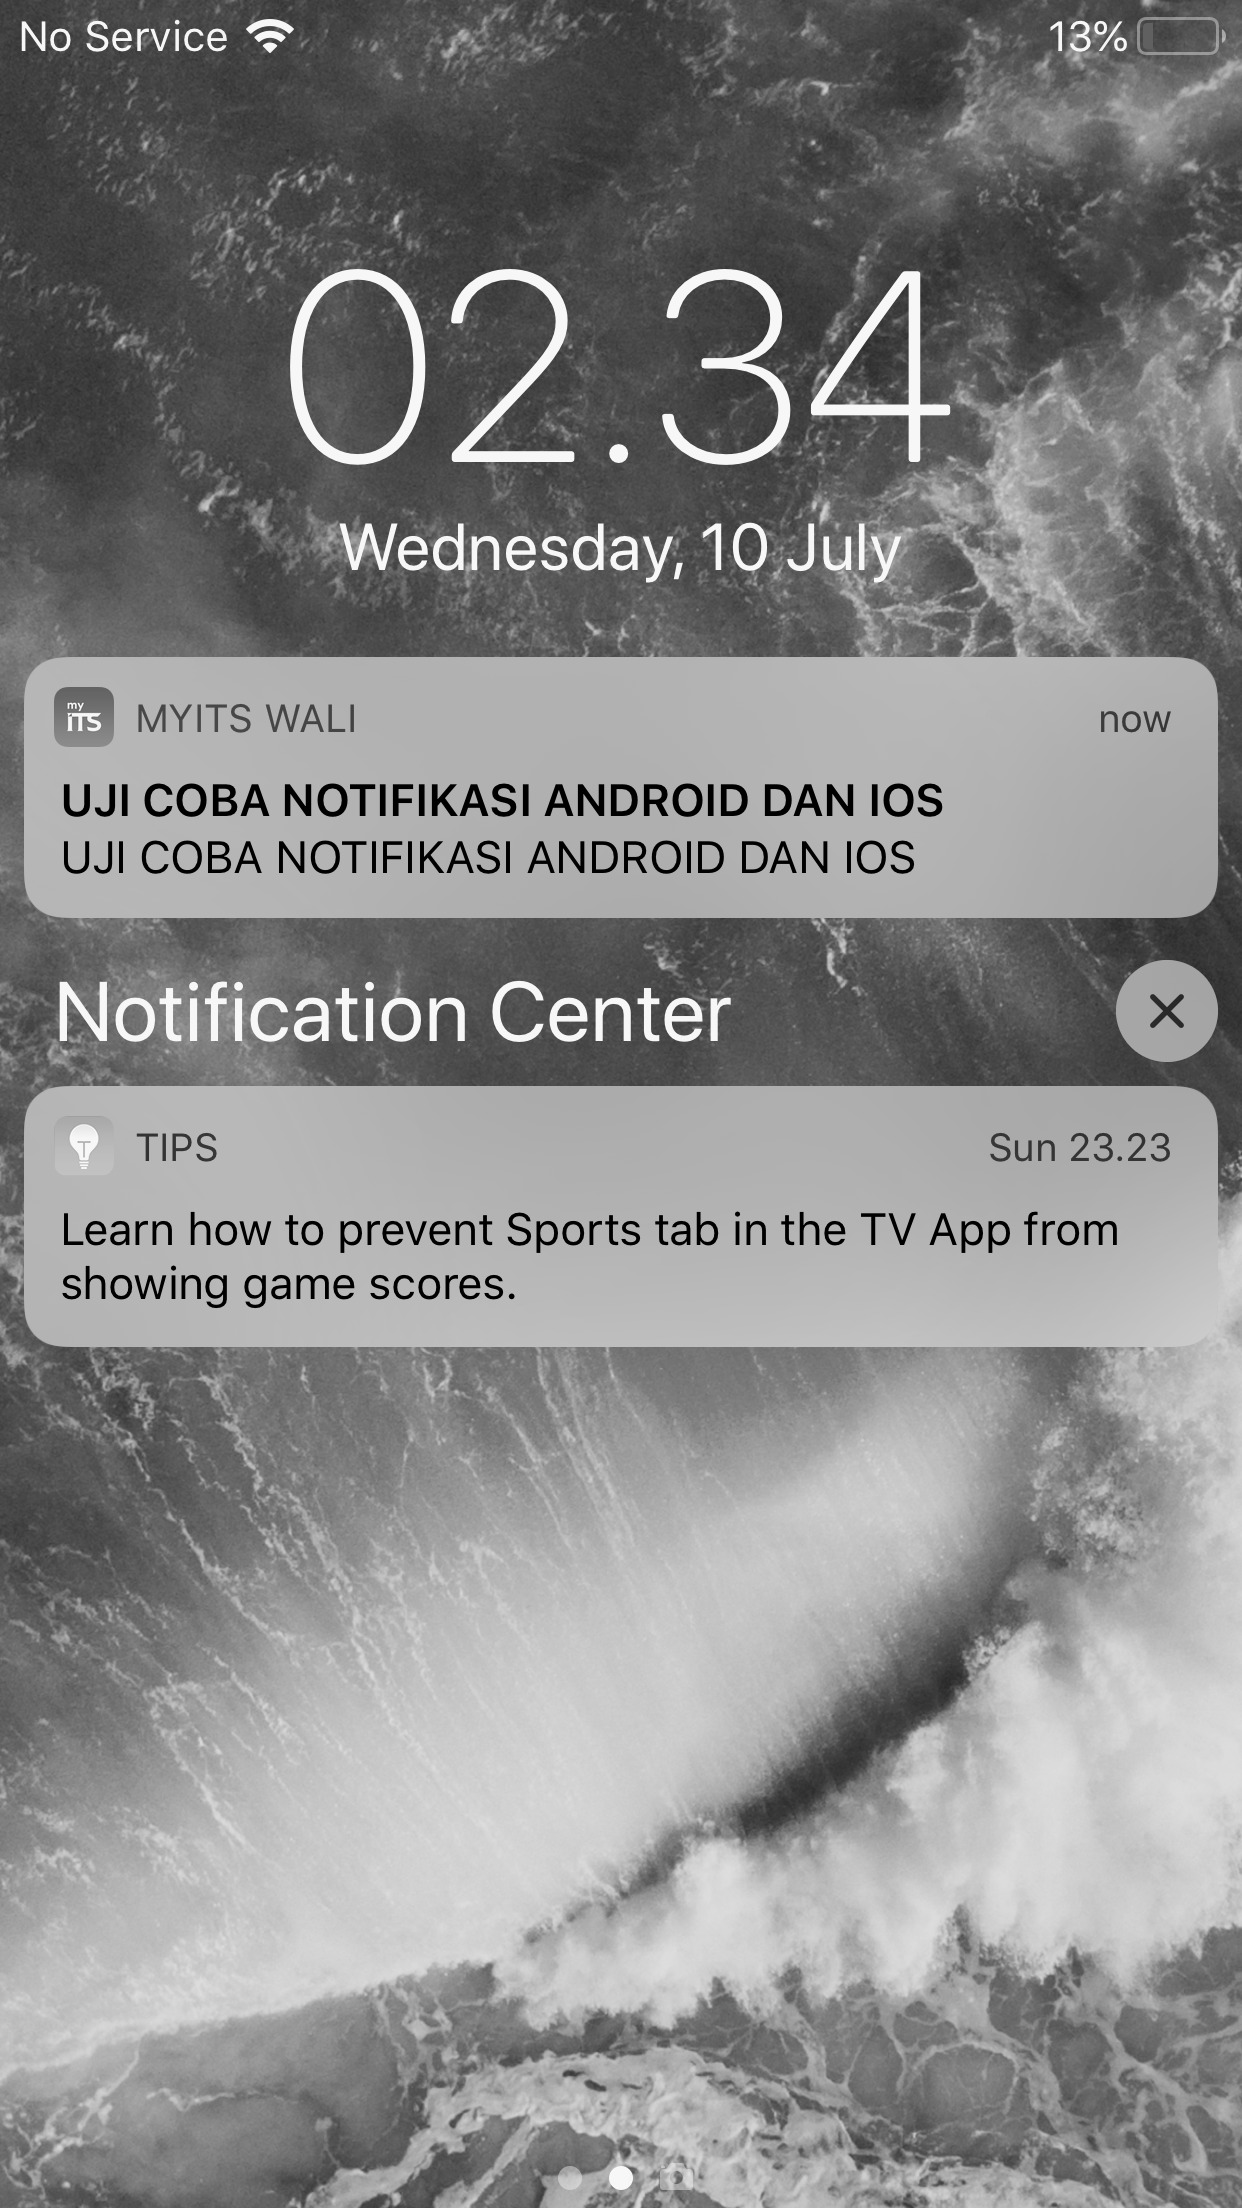
\includegraphics[width=0.4\textwidth]{bab5/img/notifikasi-ios.jpg}
	\caption{Hasil Notifikasi di Perangkat iOS} \label{f:ss_ios}
\end{figure}

\subsection{Pengujian Pengiriman Packet ke FCM}
\par Pengujian pengiriman \textit{packet} ke FCM dilakukan untuk mengetahui apakah Sender FCM berhasil mengirimkan \textit{packet} ke layanan FCM dengan tepat. Hasil uji dan notifikasi dapat dilihat pada Tabel \ref{t:uji_pengiriman_packet_fcm} dan Gambar \ref{img:notifikasi-android}.
\begin{longtable}{|>{\columncolor{lightgray}}p{3cm}|p{6.5cm}|}
	\caption{Hasil Uji Pengiriman \textit{Packet} ke FCM} \label{t:uji_pengiriman_packet_fcm} \\ \hline
	Kode & FT-04 \\ \hline
	Nama & Pengujian Pengiriman \textit{Packet} ke FCM \\ \hline
	Tujuan & Menguji apakah sistem mampu mengirim \textit{packet} lewat layanan FCM \\ \hline
	Kondisi Awal & Scheduler dan Sender FCM aktif \\ \hline
	Langkah Pengujian &  
	\begin{enumerate}
		\item Pengguna menambahkan data \textit{batch} baru untuk perangkat Android lewat halaman kirim notifikasi di modul Manajemen.
		\item 1 menit setelah waktu pengiriman \textit{batch}, notifikasi akan diterima oleh perangkat Android.
	\end{enumerate} \\ \hline
	Hasil yang diharapkan & Notifikasi diterima oleh perangkat Android \\ \hline
	Hasil yang diperoleh & Notifikasi diterima oleh perangkat Android \\ \hline
	Hasil pengujian & Berhasil \\ \hline
\end{longtable}
\begin{figure}[H]
	\centering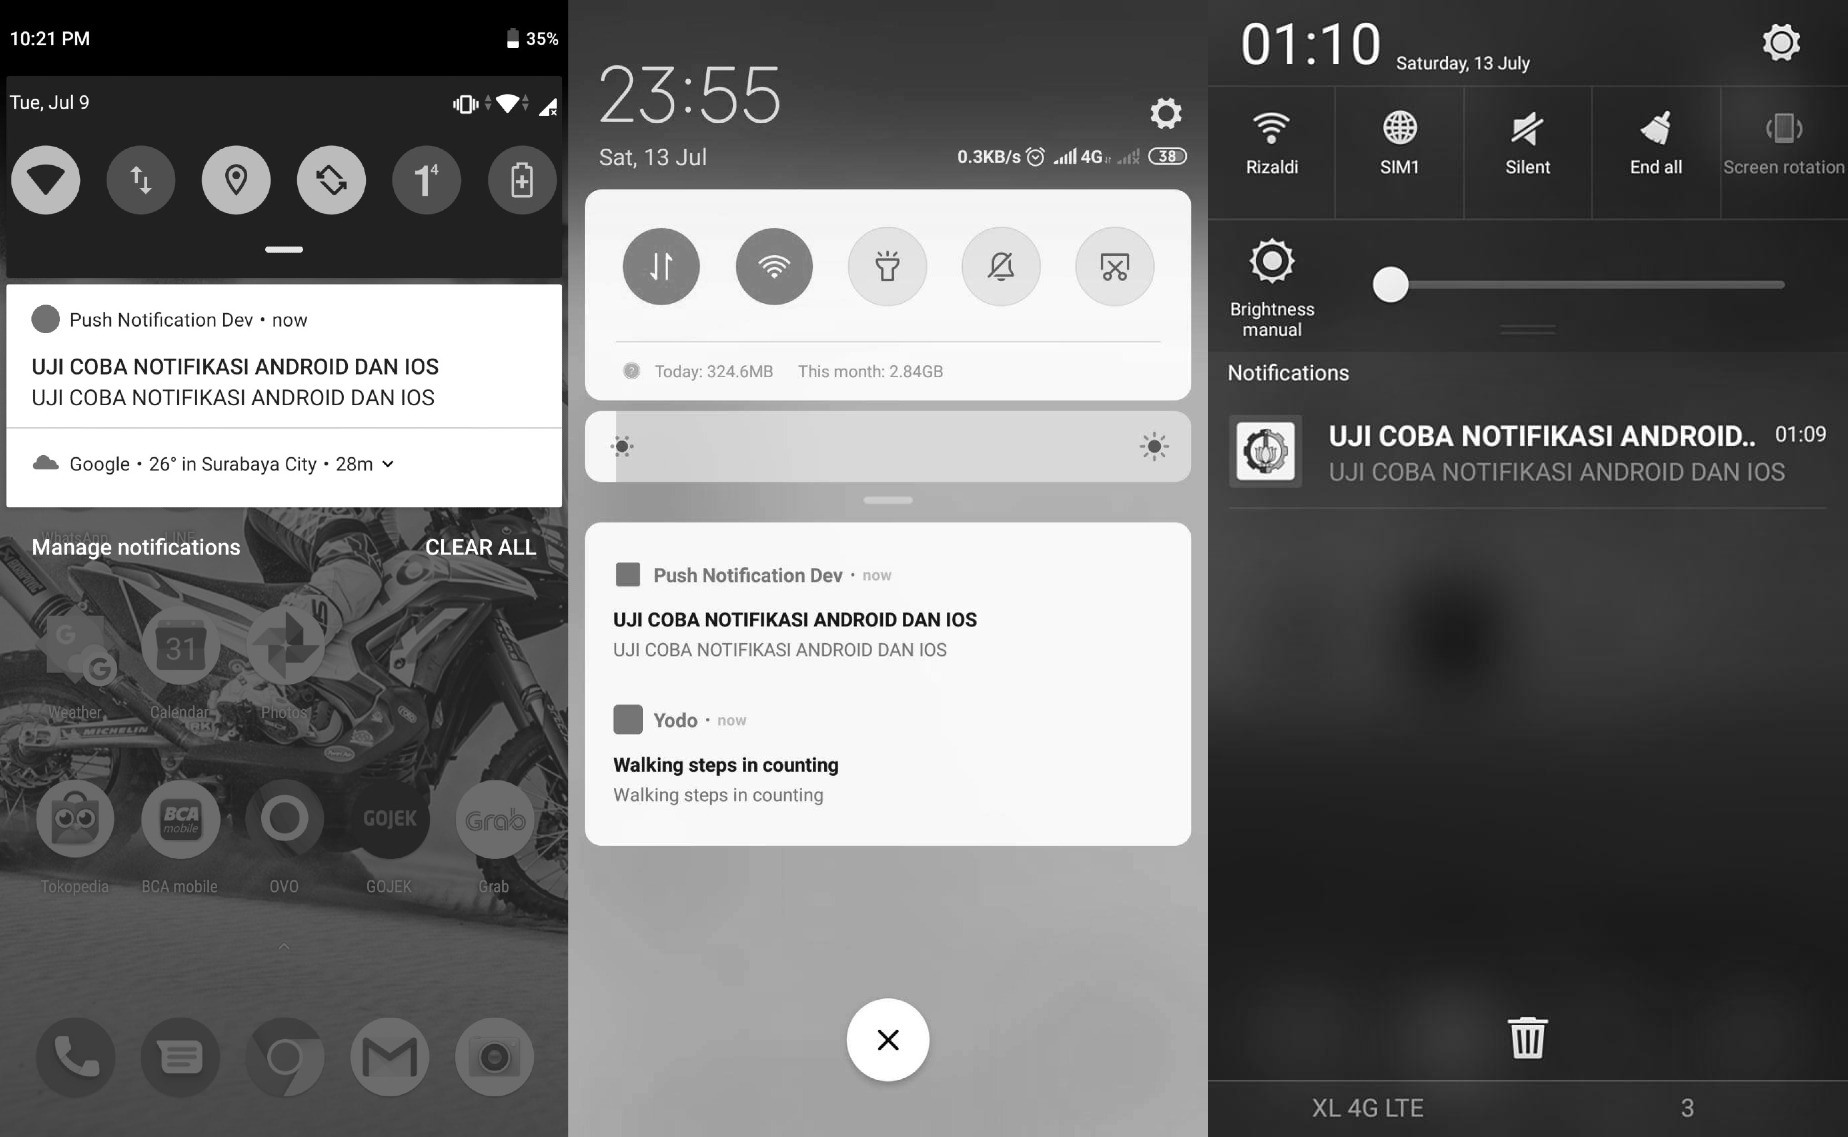
\includegraphics[width=1\textwidth]{bab5/img/notifikasi-android.jpg}
	\caption{Hasil Notifikasi di Perangkat Android 1, 2, dan 3} \label{img:notifikasi-android}
\end{figure}

\subsection{Pengujian Menampilkan Penggunaan Sumber Daya}
\par Pengujian menampilkan penggunaan sumber daya dilakukan untuk mengetahui apakah Scheduler, Sender APN, dan Sender FCM berhasil menampilkan penggunaan sumber daya dengan tepat. Hasil uji dapat dilihat pada Tabel \ref{t:uji_menampilkan_penggunaan_sumber_daya}.
\begin{longtable}{|>{\columncolor{lightgray}}p{3cm}|p{6.5cm}|}
	\caption{Hasil Uji Menampilkan Penggunaan Sumber Daya} \label{t:uji_menampilkan_penggunaan_sumber_daya} \\ \hline
	Kode & FT-05 \\ \hline
	Nama & Pengujian Menampilkan Penggunaan Sumber Daya \\ \hline
	Tujuan & Menguji apakah sistem mampu menampilkan penggunaan sumber daya \\ \hline
	Kondisi Awal & Scheduler, Sender APN, dan Sender FCM aktif \\ \hline
	Langkah Pengujian &  
	\begin{enumerate}
		\item Pengguna mengakses \textit{endpoint} /actuator/metrics/jvm.memory.used.
		\item Sistem mengembalikan metrik penggunaan memori JVM dalam bentuk JSON.
		\item Pengguna mengakses \textit{endpoint} /actuator/metrics/system.cpu.usage.
		\item Sistem mengembalikan metrik penggunaan CPU dalam bentuk JSON.
	\end{enumerate} \\ \hline
	Hasil yang diharapkan & Aplikasi menampilkan metrik penggunaan Memori dan CPU \\ \hline
	Hasil yang diperoleh & Aplikasi menampilkan metrik penggunaan Memori dan CPU \\ \hline
	Hasil pengujian & Berhasil \\ \hline
\end{longtable}

\subsection{Pengujian Menampilkan Status Kesehatan}
\par Pengujian menampilkan status kesehatan dilakukan untuk mengetahui apakah Scheduler, Sender APN, dan Sender FCM berhasil menampilkan status kesehatan dengan tepat. Hasil uji dapat dilihat pada Tabel \ref{t:uji_menampilkan_status_kesehatan}.
\begin{longtable}{|>{\columncolor{lightgray}}p{3cm}|p{6.5cm}|}
	\caption{Hasil Uji Menampilkan Status Kesehatan} \label{t:uji_menampilkan_status_kesehatan} \\ \hline
	Kode & FT-06 \\ \hline
	Nama & Pengujian Menampilkan Status Kesehatan \\ \hline
	Tujuan & Menguji apakah sistem mampu menampilkan status kesehatan \\ \hline
	Kondisi Awal & Scheduler, Sender APN, dan Sender FCM aktif \\ \hline
	Langkah Pengujian &  
	\begin{enumerate}
		\item Pengguna mengakses \textit{endpoint} /actuator/health.
		\item Sistem mengembalikan metrik kesehatan layanan sistem basis data dan antrian pesan dalam bentuk JSON.
	\end{enumerate} \\ \hline
	Hasil yang diharapkan & Sistem menampilkan status kesehatan sistem basis data dan antrian pesan \\ \hline
	Hasil yang diperoleh & Sistem menampilkan status kesehatan sistem basis data dan antrian pesan \\ \hline
	Hasil pengujian & Berhasil \\ \hline
\end{longtable}

\subsection{Pengujian Menampilkan Konfigurasi}
\par Pengujian menampilkan konfigurasi dilakukan untuk mengetahui apakah Scheduler, Sender APN, dan Sender FCM berhasil menampilkan konfigurasi dengan tepat. Hasil uji dapat dilihat pada Tabel \ref{t:uji_menampilkan_konfigurasi}.
\begin{longtable}{|>{\columncolor{lightgray}}p{3cm}|p{6.5cm}|}
	\caption{Hasil Uji Menampilkan Konfigurasi} \label{t:uji_menampilkan_konfigurasi} \\ \hline
	Kode & FT-07 \\ \hline
	Nama & Pengujian Menampilkan Konfigurasi \\ \hline
	Tujuan & Menguji apakah sistem mampu menampilkan konfigurasi \\ \hline
	Kondisi Awal & Scheduler, Sender APN, dan Sender FCM aktif \\ \hline
	Langkah Pengujian &  
	\begin{enumerate}
		\item Pengguna mengakses \textit{endpoint} /actuator/env.
		\item Sistem mengembalikan konfigurasi sistem dalam bentuk JSON.
	\end{enumerate} \\ \hline
	Hasil yang diharapkan & Sistem menampilkan konfigurasi yang digunakan \\ \hline
	Hasil yang diperoleh & Sistem menampilkan konfigurasi yang digunakan \\ \hline
	Hasil pengujian & Berhasil \\ \hline
\end{longtable}

\subsection{Pengujian Menampilkan Log}
\par Pengujian menampilkan \textit{log} dilakukan untuk mengetahui apakah Scheduler, Sender APN, dan Sender FCM berhasil menampilkan \textit{log} dengan tepat. Hasil uji dapat dilihat pada Tabel \ref{t:uji_menampilkan_log}.
\begin{longtable}{|>{\columncolor{lightgray}}p{3cm}|p{6.5cm}|}
	\caption{Hasil Uji Menampilkan \textit{Log}} \label{t:uji_menampilkan_log} \\ \hline
	Kode & FT-08 \\ \hline
	Nama & Pengujian Menampilkan \textit{Log} \\ \hline
	Tujuan & Menguji apakah sistem mampu menampilkan \textit{log} \\ \hline
	Kondisi Awal & Scheduler, Sender APN, dan Sender FCM aktif \\ \hline
	Langkah Pengujian &  
	\begin{enumerate}
		\item Pengguna mengakses \textit{endpoint} /actuator/logfile.
		\item Sistem mengembalikan isi \textit{log} sistem bentuk teks.
	\end{enumerate} \\ \hline
	Hasil yang diharapkan & Sistem menampilkan isi \textit{log} \\ \hline
	Hasil yang diperoleh & Sistem menampilkan isi \textit{log} \\ \hline
	Hasil pengujian & Berhasil \\ \hline
\end{longtable}

\section{Pengujian Non Fungsional}
\par Pengujian non fungsional dilakukan untuk mengetahui apakah sistem yang dibangun sudah memenuhi standar yang ditentukan, dari aspek performa, keandalan, ketersediaan, dan durabilitas. Skenario pengujian dilakukan dengan mengirim \textit{packet} dengan jumlah besar ke perangkat uji.

\subsection{Pengujian Performa}
\par Pengujian performa dilakukan untuk mengetahui seberapa cepat sistem dalam mengirim \textit{packet} ke layanan APNs dan FCM. Kasus uji dibagi berdasarkan jumlah \textit{packet} yang dikirim secara bersamaan, dengan pengulangan sebanyak 5 kali.
\par Metrik keberhasilan menggunakan durasi waktu pembuatan dan pengiriman \textit{packet}. Durasi pembuatan \textit{packet} dihitung dari waktu \textit{batch} tersimpan di sistem basis data, hingga waktu \textit{batch} selesai diolah. Durasi pengiriman \textit{packet} dihitung dari waktu \textit{batch} dikirim, hingga waktu \textit{packet} terakhir dikirim.

\subsubsection{Pengujian Performa untuk 2.000 Packet}
\par Skenario pengujian dilakukan dengan membuat \textit{batch} yang menargetkan 1.000 perangkat iOS dan 1.000 perangkat Android. Rincian hasil uji dapat dilihat pada Tabel \ref{t:performa-2k}.
\begin{longtable}{|p{1.5cm}|p{2cm}|p{2cm}|p{2cm}|}
	\caption{Hasil Uji Performa Pengiriman 2.000 \textit{Packet}} \label{t:performa-2k} \\ \hline
	\rowcolor{lightgray} & \multicolumn{3}{c|}{Durasi Pengolahan \textit{Packet}} \\ \hhline{~|*3{-}|}
	\rowcolor{lightgray} \multirow{-2}{*}{Kode} & Pembuatan & Pengiriman & Total \\ \hline
	NFPT-01 & 0:00:27 & 0:01:47 & 0:02:14 \\ \hline 
	NFPT-02 & 0:00:15 & 0:01:34 & 0:01:49 \\ \hline
	NFPT-03 & 0:00:28 & 0:01:50 & 0:02:18 \\ \hline
	NFPT-04 & 0:00:05 & 0:02:14 & 0:02:19 \\ \hline
	NFPT-05 & 0:00:25 & 0:01:39 & 0:02:04 \\ \hline
\end{longtable}

\subsubsection{Pengujian Performa untuk 20.000 Packet}
\par Skenario pengujian dilakukan dengan membuat \textit{batch} yang menargetkan 10.000 perangkat iOS dan 10.000 perangkat Android. Rincian hasil uji dapat dilihat pada Tabel \ref{t:performa-20k}.
\begin{longtable}{|p{1.5cm}|p{2cm}|p{2cm}|p{2cm}|}
	\caption{Hasil Uji Performa Pengiriman 20.000 \textit{Packet}} \label{t:performa-20k} \\ \hline
	\rowcolor{lightgray} & \multicolumn{3}{c|}{Durasi Pengolahan \textit{Packet}} \\ \hhline{~|*3{-}|}
	\rowcolor{lightgray} \multirow{-2}{*}{Kode} & Pembuatan & Pengiriman & Total \\ \hline
	NFPT-06 & 0:01:42 & 0:15:04 & 0:16:46 \\ \hline 
	NFPT-07 & 0:01:27 & 0:21:34 & 0:23:01 \\ \hline
	NFPT-08 & 0:00:48 & 0:12:10 & 0:12:58 \\ \hline
	NFPT-09 & 0:01:08 & 0:16:17 & 0:17:25 \\ \hline
	NFPT-10 & 0:01:02 & 0:16:17 & 0:17:18 \\ \hline
\end{longtable}

\subsubsection{Pengujian Performa untuk 200.000 Packet}
\par Skenario pengujian dilakukan dengan membuat \textit{batch} yang menargetkan 100.000 perangkat iOS dan 100.000 perangkat Android. Rincian hasil uji dapat dilihat pada Tabel \ref{t:performa-200k}.
\begin{longtable}{|p{1.5cm}|p{2cm}|p{2cm}|p{2cm}|}
\caption{Hasil Uji Performa Pengiriman 200.000 \textit{Packet}} \label{t:performa-200k} \\ \hline
\rowcolor{lightgray} & \multicolumn{3}{c|}{Durasi Pengolahan \textit{Packet}} \\ \hhline{~|*3{-}|}
\rowcolor{lightgray} \multirow{-2}{*}{Kode} & Pembuatan & Pengiriman & Total \\ \hline
	NFPT-11 & 0:11:00 & 3:06:08 & 3:17:08 \\ \hline 
	NFPT-12 & 0:10:25 & 2:44:55 & 2:55:20 \\ \hline
	NFPT-13 & 0:08:47 & 3:11:12 & 3:20:00 \\ \hline
	NFPT-14 & 0:08:39 & 2:38:49 & 2:47:28 \\ \hline
	NFPT-15 & 0:04:09 & 1:57:47 & 2:01:56 \\ \hline
\end{longtable}

\subsection{Pengujian Keandalan}
\par Pengujian keandalan dilakukan untuk mengetahui tingkat keberhasilan pengiriman \textit{packet} ke perangkat pengguna. Kasus uji dibagi berdasarkan jenis perangkat, dan jumlah \textit{packet} yang diuji, dengan pengulangan sebanyak 5 kali.

\subsubsection{Pengujian Keandalan Pengiriman Packet ke Perangkat iOS}
\par Pengujian keandalan pengiriman \textit{packet} ke perangkat iOS dilakukan untuk mengetahui tingkat keberhasilan pengiriman \textit{packet} ke layanan APNs dan perangkat iOS berdasarkan jumlah \textit{packet} yang dikirim secara bersamaan.
\par Metrik keberhasilan menggunakan jumlah \textit{packet} yang diterima oleh Sender APN, APNs dan perangkat iOS, dengan ketentuan sebagai berikut:
\begin{enumerate}
	\item Jumlah \textit{packet} yang diterima oleh Sender APN adalah jumlah \textit{packet} yang berhasil atau gagal.
	\item Jumlah \textit{packet} yang diterima oleh APNs adalah jumlah \textit{packet} yang berhasil atau gagal dengan \textit{error} ApnsClientException.
	\item Jumlah \textit{packet} yang diterima oleh perangkat iOS adalah jumlah \textit{packet} yang berhasil.
\end{enumerate}
   

\paragraph{Pengujian Keandalan Pengiriman 1.000 Packet ke Perangkat iOS}
\par Skenario pengujian dilakukan dengan membuat \textit{batch} yang menargetkan 1.000 pengguna dengan perangkat iOS. Hasil uji dapat diliat pada Tabel \ref{t:keandalan-ios-1k}.
\begin{longtable}{|p{1.5cm}|p{2cm}|p{2cm}|p{2cm}|}
	\caption{Hasil Uji Keandalan Pengiriman 1.000 \textit{Packet} ke Perangkat iOS} \label{t:keandalan-ios-1k} \\ \hline
	\rowcolor{lightgray} & \multicolumn{3}{c|}{Jumlah \textit{Packet} Diterima} \\ \hhline{~|*3{-}|}
	\rowcolor{lightgray} \multirow{-2}{*}{Kode} & Sender APN & APNs & iOS \\ \hline
	NFAT-01 & 1.000 & 1.000 & 1.000 \\ \hline
	NFAT-02 & 1.000 & 1.000 & 1.000 \\ \hline
	NFAT-03 & 1.000 & 1.000 & 1.000 \\ \hline
	NFAT-04 & 1.000 & 1.000 & 1.000 \\ \hline
	NFAT-05 & 1.000 & 1.000 & 1.000 \\ \hline
\end{longtable}

\paragraph{Pengujian Keandalan Pengiriman 10.000 Packet ke Perangkat iOS}
\par Skenario pengujian dilakukan dengan membuat \textit{batch} yang menargetkan 10.000 pengguna dengan perangkat iOS. Hasil uji dan \textit{error} yang terjadi dapat diliat pada Tabel \ref{t:keandalan-ios-10k} dan \ref{t:error-keandalan-ios-10k}.
\begin{longtable}{|p{1.5cm}|p{2cm}|p{2cm}|p{2cm}|}
	\caption{Hasil Uji Keandalan Pengiriman 10.000 \textit{Packet} ke Perangkat iOS} \label{t:keandalan-ios-10k} \\ \hline
	\rowcolor{lightgray} & \multicolumn{3}{c|}{Jumlah \textit{Packet} Diterima} \\ \hhline{~|*3{-}|}
	\rowcolor{lightgray} \multirow{-2}{*}{Kode} & Sender APN & APNs & iOS \\ \hline
	NFAT-06 & 10.000 & 10.000 & 9.984 \\ \hline
	NFAT-07 & 10.000 & 10.000 & 9.992 \\ \hline
	NFAT-08 & 10.000 & 10.000 & 9.984 \\ \hline
	NFAT-09 & 10.000 & 10.000 & 9.992 \\ \hline
	NFAT-10 & 10.000 & 10.000 & 9.984 \\ \hline
\end{longtable}
\begin{longtable}{|p{1.5cm}|p{1.5cm}|p{4cm}|}
	\caption{\textit{Error} pada Hasil Uji Keandalan Pengiriman 10.000 \textit{Packet} ke Perangkat iOS} \label{t:error-keandalan-ios-10k} \\ \hline
	\rowcolor{lightgray} Kode & Jumlah & Alasan \\ \hline
	NFAT-06 & 16 & ApnsClientException: TooManyRequests \\ \hline
	NFAT-07 & 8 & ApnsClientException: TooManyRequests \\ \hline
	NFAT-08 & 16 & ApnsClientException: TooManyRequests \\ \hline
	NFAT-09 & 8 & ApnsClientException: TooManyRequests \\ \hline
	NFAT-10 & 16 & ApnsClientException: TooManyRequests \\ \hline
\end{longtable}

\paragraph{Pengujian Keandalan Pengiriman 100.000 Packet ke Perangkat iOS}
\par Skenario pengujian dilakukan dengan membuat \textit{batch} yang menargetkan 100.000 pengguna dengan perangkat iOS. Hasil uji dan \textit{error} yang terjadi dapat diliat pada Tabel \ref{t:keandalan-ios-100k} dan \ref{t:error-keandalan-ios-100k}.
\begin{longtable}{|p{1.5cm}|p{2cm}|p{2cm}|p{2cm}|}
	\caption{Hasil Uji Keandalan Pengiriman 100.000 \textit{Packet} ke Perangkat iOS} \label{t:keandalan-ios-100k} \\ \hline
	\rowcolor{lightgray} & \multicolumn{3}{c|}{Jumlah \textit{Packet} Diterima} \\ \hhline{~|*3{-}|}
	\rowcolor{lightgray} \multirow{-2}{*}{Kode} & Sender APN & APNs & iOS \\ \hline
	NFAT-11 & 100.000 & 99.996 & 99.866 \\ \hline
	NFAT-12 & 100.000 & 100.000 & 99.848 \\ \hline
	NFAT-13 & 100.000 & 100.000 & 99.856 \\ \hline
	NFAT-14 & 100.000 & 100.000 & 99.872 \\ \hline
	NFAT-15 & 100.000 & 100.000 & 99.840 \\ \hline
\end{longtable}
\begin{longtable}{|p{1.5cm}|p{1.5cm}|p{4cm}|}
\caption{\textit{Error} pada Hasil Uji Keandalan Pengiriman 100.000 \textit{Packet} ke Perangkat iOS} \label{t:error-keandalan-ios-100k} \\ \hline
\rowcolor{lightgray} Kode & Jumlah & Alasan \\ \hline
 & 130 & ApnsClientException: TooManyRequests \\ \hhline{~|*2{-}|}
\multirow{-1}{*}{NFAT-11} & 4 & IOException: Stream closed before a reply was received \\ \hline
NFAT-12 & 152 & ApnsClientException: TooManyRequests \\ \hline
NFAT-13 & 144 & ApnsClientException: TooManyRequests \\ \hline
NFAT-14 & 128 & ApnsClientException: TooManyRequests \\ \hline
NFAT-15 & 160 & ApnsClientException: TooManyRequests \\ \hline
\end{longtable}

\subsubsection{Pengujian Keandalan Pengiriman Packet ke Perangkat Android}
\par Pengujian keandalan pengiriman \textit{packet} ke perangkat Android dilakukan untuk mengetahui tingkat keberhasilan pengiriman \textit{packet} ke layanan FCM dan perangkat Android berdasarkan jumlah \textit{packet} yang dikirim secara bersamaan.
\par Metrik keberhasilan menggunakan jumlah \textit{packet} yang diterima oleh Sender FCM, FCM dan perangkat Android 1, 2, dan 3, dengan ketentuan sebagai berikut:
\begin{enumerate}
	\item Jumlah \textit{packet} yang diterima oleh Sender FCM adalah jumlah \textit{packet} yang berhasil atau gagal.
	\item Jumlah \textit{packet} yang diterima oleh FCM adalah jumlah \textit{packet} yang berhasil atau gagal dengan \textit{error} FirebaseMessagingException.
	\item Jumlah \textit{packet} yang diterima oleh perangkat Android adalah jumlah \textit{packet} yang berhasil.
\end{enumerate}


\paragraph{Pengujian Keandalan Pengiriman 1.000 Packet ke Perangkat Android}
\par Skenario pengujian dilakukan dengan membuat \textit{batch} yang menargetkan 1.000 pengguna dengan perangkat Android. Hasil uji dapat diliat pada Tabel \ref{t:keandalan-android-1k}.
\begin{longtable}{|p{1.5cm}|p{2cm}|p{1.5cm}|p{1cm}|p{1cm}|p{1cm}|}
	\caption{Hasil Uji Keandalan Pengiriman 1.000 \textit{Packet} ke Perangkat Android} \label{t:keandalan-android-1k} \\ \hline
	\rowcolor{lightgray} & \multicolumn{5}{c|}{Jumlah \textit{Packet} Diterima} \\ \hhline{~|*5{-}|}
	\rowcolor{lightgray} & & & \multicolumn{3}{c|}{Android} \\ \hhline{~~~|*3{-}|}
	\rowcolor{lightgray} \multirow{-3}{*}{Kode} & \multirow{-2}{*}{Sender FCM} & \multirow{-2}{*}{FCM} & 1 & 2 & 3 \\ \hline
	NFAT-16 & 1.000 & 1.000 & 333 & 334 & 333 \\ \hline
	NFAT-17 & 1.000 & 1.000 & 333 & 334 & 333 \\ \hline
	NFAT-18 & 1.000 & 1.000 & 333 & 334 & 333 \\ \hline
	NFAT-19 & 1.000 & 1.000 & 333 & 334 & 333 \\ \hline
	NFAT-20 & 1.000 & 1.000 & 333 & 334 & 333 \\ \hline
\end{longtable}

\paragraph{Pengujian Keandalan Pengiriman 10.000 Packet ke Perangkat Android}
\par Skenario pengujian dilakukan dengan membuat \textit{batch} yang menargetkan 10.000 pengguna dengan perangkat Android. Hasil uji dapat diliat pada Tabel \ref{t:keandalan-android-10k}.
\begin{longtable}{|p{1.5cm}|p{2cm}|p{1.5cm}|p{1cm}|p{1cm}|p{1cm}|}
	\caption{Hasil Uji Keandalan Pengiriman 10.000 \textit{Packet} ke Perangkat Android} \label{t:keandalan-android-10k} \\ \hline
	\rowcolor{lightgray} & \multicolumn{5}{c|}{Jumlah \textit{Packet} Diterima} \\ \hhline{~|*5{-}|}
	\rowcolor{lightgray} & & & \multicolumn{3}{c|}{Android} \\ \hhline{~~~|*3{-}|}
	\rowcolor{lightgray} \multirow{-3}{*}{Kode} & \multirow{-2}{*}{Sender FCM} & \multirow{-2}{*}{FCM} & 1 & 2 & 3 \\ \hline
	NFAT-21 & 10.000 & 10.000 & 3.333 & 3.334 & 3.333 \\ \hline
	NFAT-22 & 10.000 & 10.000 & 3.333 & 3.334 & 3.333 \\ \hline
	NFAT-23 & 10.000 & 10.000 & 3.333 & 3.334 & 3.333 \\ \hline
	NFAT-24 & 10.000 & 10.000 & 3.333 & 3.334 & 3.333 \\ \hline
	NFAT-25 & 10.000 & 10.000 & 3.333 & 3.334 & 3.333 \\ \hline
\end{longtable}

\paragraph{Pengujian Keandalan Pengiriman 100.000 Packet ke Perangkat Android}
\par Skenario pengujian dilakukan dengan membuat \textit{batch} yang menargetkan 100.000 pengguna dengan perangkat Android. Hasil uji dan \textit{error} yang terjadi dapat diliat pada Tabel \ref{t:keandalan-android-100k} dan \ref{t:error-keandalan-android-100k}.
\begin{longtable}{|p{1.5cm}|p{2cm}|p{1.5cm}|p{1cm}|p{1cm}|p{1cm}|}
	\caption{Hasil Uji Keandalan Pengiriman 100.000 \textit{Packet} ke Perangkat Android} \label{t:keandalan-android-100k} \\ \hline
	\rowcolor{lightgray} & \multicolumn{5}{c|}{Jumlah \textit{Packet} Diterima} \\ \hhline{~|*5{-}|}
	\rowcolor{lightgray} & & & \multicolumn{3}{c|}{Android} \\ \hhline{~~~|*3{-}|}
	\rowcolor{lightgray} \multirow{-3}{*}{Kode} & \multirow{-2}{*}{Sender FCM} & \multirow{-2}{*}{FCM} & 1 & 2 & 3 \\ \hline
	NFAT-21 & 100.000 & 100.000 & 33.333 & 33.334 & 33.333 \\ \hline
	NFAT-22 & 100.000 & 100.000 & 33.333 & 33.334 & 33.333 \\ \hline
	NFAT-23 & 100.000 & 100.000 & 33.333 & 33.334 & 33.333 \\ \hline
	NFAT-24 & 100.000 & 100.000 & 33.333 & 33.333 & 33.333 \\ \hline
	NFAT-25 & 100.000 & 100.000 & 33.333 & 33.334 & 33.333 \\ \hline
\end{longtable}
\begin{longtable}{|p{1.5cm}|p{1.5cm}|p{5cm}|}
	\caption{\textit{Error} pada Hasil Uji Keandalan Pengiriman 100.000 \textit{Packet} ke Perangkat Android} \label{t:error-keandalan-android-100k} \\ \hline
	\rowcolor{lightgray} Kode & Jumlah & Alasan \\ \hline
	NFAT-24 & 1 & FirebaseMessagingException: The service is currently unavailable. \\ \hline
\end{longtable}

\subsection{Pengujian Ketersediaan}
\par Pengujian ketersediaan dilakukan untuk mengetahui apakah sistem tetap bekerja normal saat sedang mengirimkan \textit{packet} dalam jumlah besar.
\par Metrik keberhasilan menggunakan jumlah server mengalami \textit{down} (berhenti beroperasi). Pengecekan kondisi \textit{down} dilakukan dengan mengecek status kesehatan lewat API Actuator setiap 15 menit.

\subsubsection{Pengujian Ketersediaan untuk Pengiriman 2.000 Packet}
\par Skenario pengujian dilakukan dengan membuat \textit{batch} yang menargetkan 1.000 perangkat iOS dan 1.000 perangkat Android. Rincian hasil uji dapat dilihat pada Tabel \ref{t:ketersediaan-2k}.
\begin{longtable}{|p{1.5cm}|p{2cm}|p{2cm}|p{2cm}|}
	\caption{Hasil Uji Ketersediaan Layanan untuk Pengiriman 2.000 \textit{Packet}} \label{t:ketersediaan-2k} \\ \hline
	\rowcolor{lightgray} & \multicolumn{3}{c|}{Jumlah \textit{Down}} \\ \hhline{~|*3{-}|}
	\rowcolor{lightgray} \multirow{-2}{*}{Kode}  & Scheduler & Sender APN & Sender FCM \\ \hline
	NFTT-01 & 0 & 0 & 0 \\ \hline
	NFTT-02 & 0 & 0 & 0 \\ \hline
	NFTT-03 & 0 & 0 & 0 \\ \hline
	NFTT-04 & 0 & 0 & 0 \\ \hline
	NFTT-05 & 0 & 0 & 0 \\ \hline
\end{longtable}

\subsubsection{Pengujian Ketersediaan untuk Pengiriman 20.000 Packet}
\par Skenario pengujian dilakukan dengan membuat \textit{batch} yang menargetkan 10.000 perangkat iOS dan 10.000 perangkat Android. Rincian hasil uji dapat dilihat pada Tabel \ref{t:ketersediaan-20k}.
\begin{longtable}{|p{1.5cm}|p{2cm}|p{2cm}|p{2cm}|}
	\caption{Hasil Uji Ketersediaan Layanan untuk Pengiriman 20.000 \textit{Packet}} \label{t:ketersediaan-20k} \\ \hline
	\rowcolor{lightgray} & \multicolumn{3}{c|}{Jumlah \textit{Down}} \\ \hhline{~|*3{-}|}
	\rowcolor{lightgray} \multirow{-2}{*}{Kode}  & Scheduler & Sender APN & Sender FCM \\ \hline
	NFTT-06 & 0 & 0 & 0 \\ \hline
	NFTT-07 & 0 & 0 & 0 \\ \hline
	NFTT-08 & 0 & 0 & 0 \\ \hline
	NFTT-09 & 0 & 0 & 0 \\ \hline
	NFTT-10 & 0 & 0 & 0 \\ \hline
\end{longtable}

\subsubsection{Pengujian Ketersediaan untuk Pengiriman 200.000 Packet}
\par Skenario pengujian dilakukan dengan membuat \textit{batch} yang menargetkan 100.000 perangkat iOS dan 100.000 perangkat Android. Rincian hasil uji dapat dilihat pada Tabel \ref{t:ketersediaan-200k}.
\begin{longtable}{|p{1.5cm}|p{2cm}|p{2cm}|p{2cm}|}
	\caption{Hasil Uji Ketersediaan Layanan untuk Pengiriman 200.000 \textit{Packet}} \label{t:ketersediaan-200k} \\ \hline
	\rowcolor{lightgray} & \multicolumn{3}{c|}{Jumlah \textit{Down}} \\ \hhline{~|*3{-}|}
	\rowcolor{lightgray} \multirow{-2}{*}{Kode}  & Scheduler & Sender APN & Sender FCM \\ \hline
	NFTT-11 & 0 & 0 & 0 \\ \hline
	NFTT-12 & 0 & 0 & 0 \\ \hline
	NFTT-13 & 0 & 0 & 0 \\ \hline
	NFTT-14 & 0 & 0 & 0 \\ \hline
	NFTT-15 & 0 & 0 & 0 \\ \hline
\end{longtable}

\subsection{Pengujian Durabilitas}
\par Pengujian durabilitas dilakukan untuk mengetahui apakah sistem tetap bekerja normal saat salah satu layanan mati. Pengujian dibagi menjadi 2 skenario, yaitu saat Sender APN dimatikan dan Sender FCM dimatikan.

\subsubsection{Pengujian Mematikan Sementara Sender APN}
\par Pengujian mematikan sementara Sender APN dilakukan dengan cara mematikan Sender APN selama 5 menit ditengah proses pengiriman \textit{packet}. Hasil uji dapat dilihat pada Tabel \ref{t:nft_sender_apn_mati}.
\begin{longtable}{|>{\columncolor{lightgray}}p{3cm}|p{6.5cm}|}
	\caption{Hasil Uji Mematikan Sementara Sender APN} \label{t:nft_sender_apn_mati} \\ \hline
	Kode & NFDT-01 \\ \hline
	Nama & Pengujian Mematikan Sementara Sender APN \\ \hline
	Tujuan & Mengetahui apakah sistem mampu mengirimkan \textit{push notification} jika Sender APN mati sementara \\ \hline
	Kondisi Awal & Sistem dalam keadaan berjalan \\ \hline
	Langkah Pengujian &  
	\begin{enumerate}
		\item Aktor membuat \textit{batch} baru lewat halaman kirim notifikasi pada modul manajemen.
		\item Sender APN dimatikan selama 5 menit.
	\end{enumerate} \\ \hline
	Hasil yang diharapkan & Notifikasi diterima oleh perangkat iOS \\ \hline
	Hasil yang diperoleh & Notifikasi diterima oleh perangkat iOS \\ \hline
	Hasil pengujian & Berhasil \\ \hline
\end{longtable}

\subsubsection{Pengujian Mematikan Sementara Sender FCM}
\par Pengujian mematikan sementara Sender FCM dilakukan dengan cara mematikan Sender FCM selama 5 menit ditengah proses pengiriman \textit{packet}. Hasil uji dapat dilihat pada Tabel \ref{t:nft_sender_fcm_mati}.
\begin{longtable}{|>{\columncolor{lightgray}}p{3cm}|p{6.5cm}|}
	\caption{Hasil Uji Mematikan Sementara Sender FCM} \label{t:nft_sender_fcm_mati} \\ \hline
	Kode & NFDT-02 \\ \hline
	Nama & Pengujian Mematikan Sementara Sender FCM \\ \hline
	Tujuan & Mengetahui apakah sistem mampu mengirimkan \textit{push notification} jika Sender FCM mati sementara \\ \hline
	Kondisi Awal & Sistem dalam keadaan berjalan \\ \hline
	Langkah Pengujian &  
	\begin{enumerate}
		\item Aktor membuat \textit{batch} baru lewat halaman kirim notifikasi pada modul manajemen.
		\item Sender FCM dimatikan selama 5 menit.
	\end{enumerate} \\ \hline
	Hasil yang diharapkan & Notifikasi diterima oleh perangkat Android \\ \hline
	Hasil yang diperoleh & Notifikasi diterima oleh perangkat Android \\ \hline
	Hasil pengujian & Berhasil \\ \hline
\end{longtable}

\section{Evaluasi Hasil Pengujian}
\par Evaluasi hasil pengujian membahas apakah kebutuhan fungsional dan non fungsional aplikasi sudah terpenuhi berdasarkan hasil pengujian yang dilakukan, penyebab kegagalan pada saat pengujian, serta perbandingan dengan aplikasi sebelumnya.

\subsection{Evaluasi Hasil Pengujian Fungsional}
\par Berdasarkan hasil uji, Aplikasi Push Notification Terpusat yang dibangun pada tugas akhir ini sudah memenuhi semua kebutuhan fungsional dan non fungsional yang ada. Rangkuman hasil uji untuk kebutuhan fungsional dapat dilihat pada Tabel \ref{t:eval_f}.
\begin{longtable}{|p{1.5cm}|p{3cm}|p{1.5cm}|p{1.5cm}|}
	\caption{Rangkuman Hasil Uji Fungsional} \label{t:eval_f} \\ \hline
	\rowcolor{lightgray} Kode Kebutuhan & Nama Kebutuhan & Kode Uji & Hasil \\ \hline
	F-01 & Pembuatan \textit{Packet} & FT-01 & Berhasil \\ \hline
	F-02 & Menambahkan \textit{Packet} ke Antrian & FT-02 & Berhasil \\ \hline
	F-03 & Pengiriman \textit{Packet} ke APNs & FT-03 & Berhasil \\ \hline
	F-04 & Pengiriman \textit{Packet} ke FCM & FT-04 & Berhasil \\ \hline
	F-05 & Menampilkan Penggunaan Sumber Daya & FT-05 & Berhasil \\ \hline
	F-06 & Menampilkan Status Kesehatan & FT-06 & Berhasil \\ \hline
	F-07 & Menampilkan Konfigurasi & FT-07 & Berhasil \\ \hline
	F-08 & Menampilkan \textit{Log} & FT-08 & Berhasil \\ \hline
\end{longtable}

\subsection{Evaluasi Hasil Pengujian Non Fungsional}
%TODO

\subsubsection{Evaluasi Hasil Pengujian Performa}
%TODO

\subsubsection{Evaluasi Hasil Pengujian Keandalan}
%TODO

\subsubsection{Evaluasi Hasil Pengujian Ketersediaan}
%TODO

\subsubsection{Evaluasi Hasil Pengujian Durabilitas}
%TODO

% \begin{longtable}{|p{1.5cm}|p{2cm}|p{3cm}|p{1.5cm}|}
%	\caption{Rangkuman Hasil Uji Non Fungsional} \label{t:eval_nf} \\ \hline
%	\rowcolor{lightgray} Kode Kebutuhan & Aspek & Kode Uji & Hasil \\ \hline
%	NF-01 & Performa & NFT-01, NFT-02, NFT-03 & Terpenuhi \\ \hline
%	NF-02 & Keandalan & NFT-04, NFT-05, NFT-06, NFT-07, NFT-08, NFT-09 & Terpenuhi \\ \hline
%	NF-03 & Ketersediaan & NFT-10, NFT-11, NFT-12 & Terpenuhi \\ \hline
%	NF-04 & Durabilitas & NFT-13, NFT-14 & Terpenuhi \\ \hline
%\end{longtable}

 \cleardoublepage
    \chapter{KESIMPULAN DAN SARAN}
\par Bab ini membahas kesimpulan yang diperoleh selama pengerjaan tugas akhir dan saran yang dapat dilakukan untuk mengembangkan tugas akhir ini.

\section{Kesimpulan}
\begin{enumerate}
	\item Implementasi antrian pesan dengan Kafka dapat dilakukan dengan menggunakan Docker untuk menjalankan Kafka, dan kerangka kerja Spring untuk mengirim dan mengambil pesan dari antrian.
	\item Implementasi penjadwalan pengiriman \textit{push notification} dapat dilakukan dengan membuat layanan penjadwalan yang memeriksa sistem basis data setiap 30 detik.
	\item Implementasi pengiriman \textit{push notification} ke perangkat Android dapat dilakukan dengan mengirim \textit{request push notification} ke layanan FCM, sedangkan pengiriman ke perangkat iOS dapat dilakukan dengan mengirim \textit{request push notification} ke layanan APNs.
	\item Implementasi pemantauan aplikasi dapat dilakukan dengan menggunakan pustaka Actuator.
\end{enumerate}

\section{Saran}
\begin{enumerate}
    \item Memperbarui data perangkat yang sudah tidak aktif berdasarkan \textit{response} dari layanan APNs dan FCM ketika mengirim notifikasi.
    \item Menambahkan indeks untuk mempercepat pencarian di sistem basis data.
\end{enumerate}
 \cleardoublepage

    \backmatter
    \printbibliography
    \chapter{Lampiran D: Skema JSON Packet} \label{lampiran:skema-json-packet}
\lstinputlisting[label=json:packet, caption=Skema JSON \textit{Packet}] {penutup/lampiran/d/packet.json}

    \chapter{Lampiran D: Skema JSON Packet} \label{lampiran:skema-json-packet}
\lstinputlisting[label=json:packet, caption=Skema JSON \textit{Packet}] {penutup/lampiran/d/packet.json}

    \chapter{Lampiran D: Skema JSON Packet} \label{lampiran:skema-json-packet}
\lstinputlisting[label=json:packet, caption=Skema JSON \textit{Packet}] {penutup/lampiran/d/packet.json}

    \chapter{Lampiran D: Skema JSON Packet} \label{lampiran:skema-json-packet}
\lstinputlisting[label=json:packet, caption=Skema JSON \textit{Packet}] {penutup/lampiran/d/packet.json}

    
\chapter{BIODATA PENULIS}

\begin{wrapfigure}{l}{0.3\textwidth}
	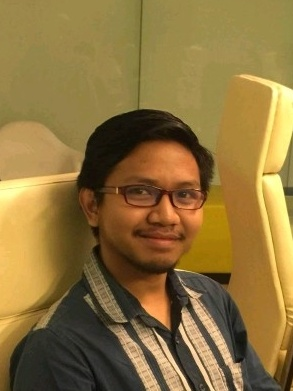
\includegraphics[height=0.25\textheight]{figures/william.jpg}
\end{wrapfigure}

Penulis bernama \penulis, lahir di Jakarta pada tanggal 03 Mei 1997.
Penulis telah menjalani masa pendidikan di Sekolah Dasar An-Nisaa pada tahun 2003 hingga 2009,
Sekolah Menengah Pertama Al-Azhar Kembangan pada tahun 2009 hingga 2012,
dan Sekolah Menengah Atas Al-Azhar Pusat Jakarta pada tahun 2012 hingga 2015.
Pada masa penulisan, penulis sedang menempuh masa studi S1 tahun ketiga di \jurusan, \fakultas,
Institut Teknologi Sepuluh Nopember.

Selama masa studi S1, penulis memiliki ketertarikan yang dalam mengenai Algoritma dan Pemrograman dan
Rancang bangun aplikasi situs web.
Penulis pernah menjadi asisten dosen pada mata kuliah Dasar Pemrograman dan Struktur Data.
Selain itu, penulis memiliki pengalaman magang di PT. Trinusa Travelindo, PT. Sumber Cipta Multiniaga,
dan PT. Stoqo Teknologi Indonesia.

Di luar kesibukan akademik, penulis cukup aktif dalam organisasi baik dari dalam maupun luar jurusan.
Penulis dapat dihubungi melalui surel di \href{mailto:irsyad.rizaldi97@gmail.com}{irsyad.rizaldi97@gmail.com}.
\end{document}